% Options for packages loaded elsewhere
\PassOptionsToPackage{unicode}{hyperref}
\PassOptionsToPackage{hyphens}{url}
\PassOptionsToPackage{dvipsnames,svgnames,x11names}{xcolor}
%
\documentclass[
  10pt,
  ignorenonframetext,
]{beamer}
\usepackage{pgfpages}
\setbeamertemplate{caption}[numbered]
\setbeamertemplate{caption label separator}{: }
\setbeamercolor{caption name}{fg=normal text.fg}
\beamertemplatenavigationsymbolsempty
% Prevent slide breaks in the middle of a paragraph
\widowpenalties 1 10000
\raggedbottom
\setbeamertemplate{part page}{
  \centering
  \begin{beamercolorbox}[sep=16pt,center]{part title}
    \usebeamerfont{part title}\insertpart\par
  \end{beamercolorbox}
}
\setbeamertemplate{section page}{
  \centering
  \begin{beamercolorbox}[sep=12pt,center]{part title}
    \usebeamerfont{section title}\insertsection\par
  \end{beamercolorbox}
}
\setbeamertemplate{subsection page}{
  \centering
  \begin{beamercolorbox}[sep=8pt,center]{part title}
    \usebeamerfont{subsection title}\insertsubsection\par
  \end{beamercolorbox}
}
\AtBeginPart{
  \frame{\partpage}
}
\AtBeginSection{
  \ifbibliography
  \else
    \frame{\sectionpage}
  \fi
}
\AtBeginSubsection{
  \frame{\subsectionpage}
}
\usepackage{amsmath,amssymb}
\usepackage{iftex}
\ifPDFTeX
  \usepackage[T1]{fontenc}
  \usepackage[utf8]{inputenc}
  \usepackage{textcomp} % provide euro and other symbols
\else % if luatex or xetex
  \usepackage{unicode-math} % this also loads fontspec
  \defaultfontfeatures{Scale=MatchLowercase}
  \defaultfontfeatures[\rmfamily]{Ligatures=TeX,Scale=1}
\fi
\usepackage{lmodern}
\usetheme[]{Frankfurt}
\usecolortheme{beaver}
\ifPDFTeX\else
  % xetex/luatex font selection
  \setmathfont[]{ccmath}
\fi
% Use upquote if available, for straight quotes in verbatim environments
\IfFileExists{upquote.sty}{\usepackage{upquote}}{}
\IfFileExists{microtype.sty}{% use microtype if available
  \usepackage[]{microtype}
  \UseMicrotypeSet[protrusion]{basicmath} % disable protrusion for tt fonts
}{}
\makeatletter
\@ifundefined{KOMAClassName}{% if non-KOMA class
  \IfFileExists{parskip.sty}{%
    \usepackage{parskip}
  }{% else
    \setlength{\parindent}{0pt}
    \setlength{\parskip}{6pt plus 2pt minus 1pt}}
}{% if KOMA class
  \KOMAoptions{parskip=half}}
\makeatother
\usepackage{xcolor}
\newif\ifbibliography
\usepackage{color}
\usepackage{fancyvrb}
\newcommand{\VerbBar}{|}
\newcommand{\VERB}{\Verb[commandchars=\\\{\}]}
\DefineVerbatimEnvironment{Highlighting}{Verbatim}{commandchars=\\\{\}}
% Add ',fontsize=\small' for more characters per line
\usepackage{framed}
\definecolor{shadecolor}{RGB}{35,38,41}
\newenvironment{Shaded}{\begin{snugshade}}{\end{snugshade}}
\newcommand{\AlertTok}[1]{\textcolor[rgb]{0.58,0.85,0.30}{\textbf{\colorbox[rgb]{0.30,0.12,0.14}{#1}}}}
\newcommand{\AnnotationTok}[1]{\textcolor[rgb]{0.25,0.50,0.35}{#1}}
\newcommand{\AttributeTok}[1]{\textcolor[rgb]{0.16,0.50,0.73}{#1}}
\newcommand{\BaseNTok}[1]{\textcolor[rgb]{0.96,0.45,0.00}{#1}}
\newcommand{\BuiltInTok}[1]{\textcolor[rgb]{0.50,0.55,0.55}{#1}}
\newcommand{\CharTok}[1]{\textcolor[rgb]{0.24,0.68,0.91}{#1}}
\newcommand{\CommentTok}[1]{\textcolor[rgb]{0.48,0.49,0.49}{#1}}
\newcommand{\CommentVarTok}[1]{\textcolor[rgb]{0.50,0.55,0.55}{#1}}
\newcommand{\ConstantTok}[1]{\textcolor[rgb]{0.15,0.68,0.68}{\textbf{#1}}}
\newcommand{\ControlFlowTok}[1]{\textcolor[rgb]{0.99,0.74,0.29}{\textbf{#1}}}
\newcommand{\DataTypeTok}[1]{\textcolor[rgb]{0.16,0.50,0.73}{#1}}
\newcommand{\DecValTok}[1]{\textcolor[rgb]{0.96,0.45,0.00}{#1}}
\newcommand{\DocumentationTok}[1]{\textcolor[rgb]{0.64,0.20,0.25}{#1}}
\newcommand{\ErrorTok}[1]{\textcolor[rgb]{0.85,0.27,0.33}{\underline{#1}}}
\newcommand{\ExtensionTok}[1]{\textcolor[rgb]{0.00,0.60,1.00}{\textbf{#1}}}
\newcommand{\FloatTok}[1]{\textcolor[rgb]{0.96,0.45,0.00}{#1}}
\newcommand{\FunctionTok}[1]{\textcolor[rgb]{0.56,0.27,0.68}{#1}}
\newcommand{\ImportTok}[1]{\textcolor[rgb]{0.15,0.68,0.38}{#1}}
\newcommand{\InformationTok}[1]{\textcolor[rgb]{0.77,0.36,0.00}{#1}}
\newcommand{\KeywordTok}[1]{\textcolor[rgb]{0.81,0.81,0.76}{\textbf{#1}}}
\newcommand{\NormalTok}[1]{\textcolor[rgb]{0.81,0.81,0.76}{#1}}
\newcommand{\OperatorTok}[1]{\textcolor[rgb]{0.81,0.81,0.76}{#1}}
\newcommand{\OtherTok}[1]{\textcolor[rgb]{0.15,0.68,0.38}{#1}}
\newcommand{\PreprocessorTok}[1]{\textcolor[rgb]{0.15,0.68,0.38}{#1}}
\newcommand{\RegionMarkerTok}[1]{\textcolor[rgb]{0.16,0.50,0.73}{\colorbox[rgb]{0.08,0.19,0.26}{#1}}}
\newcommand{\SpecialCharTok}[1]{\textcolor[rgb]{0.24,0.68,0.91}{#1}}
\newcommand{\SpecialStringTok}[1]{\textcolor[rgb]{0.85,0.27,0.33}{#1}}
\newcommand{\StringTok}[1]{\textcolor[rgb]{0.96,0.31,0.31}{#1}}
\newcommand{\VariableTok}[1]{\textcolor[rgb]{0.15,0.68,0.68}{#1}}
\newcommand{\VerbatimStringTok}[1]{\textcolor[rgb]{0.85,0.27,0.33}{#1}}
\newcommand{\WarningTok}[1]{\textcolor[rgb]{0.85,0.27,0.33}{#1}}
\usepackage{graphicx}
\makeatletter
\def\maxwidth{\ifdim\Gin@nat@width>\linewidth\linewidth\else\Gin@nat@width\fi}
\def\maxheight{\ifdim\Gin@nat@height>\textheight\textheight\else\Gin@nat@height\fi}
\makeatother
% Scale images if necessary, so that they will not overflow the page
% margins by default, and it is still possible to overwrite the defaults
% using explicit options in \includegraphics[width, height, ...]{}
\setkeys{Gin}{width=\maxwidth,height=\maxheight,keepaspectratio}
% Set default figure placement to htbp
\makeatletter
\def\fps@figure{htbp}
\makeatother
\setlength{\emergencystretch}{3em} % prevent overfull lines
\providecommand{\tightlist}{%
  \setlength{\itemsep}{0pt}\setlength{\parskip}{0pt}}
\setcounter{secnumdepth}{-\maxdimen} % remove section numbering
\ifLuaTeX
\usepackage[bidi=basic]{babel}
\else
\usepackage[bidi=default]{babel}
\fi
\babelprovide[main,import]{british}
% get rid of language-specific shorthands (see #6817):
\let\LanguageShortHands\languageshorthands
\def\languageshorthands#1{}
\usepackage{amsmath,amsfonts,fancyhdr,float,array,amsthm}
\usepackage[ligature,inference,shorthand]{semantic}
\usepackage[autostyle=true]{csquotes}
\floatplacement{figure}{H}
\usepackage{listings}
\lstset{basicstyle=\ttfamily,
  showstringspaces=false,
  commentstyle=\color{red},
  keywordstyle=\color{blue}
}
\newcommand*{\defeq}{\stackrel{\text{def}}{=}}
\newcommand{\blue}[1]{\textcolor{blue}{#1}}
\newcommand{\red}[1]{\textcolor{red}{#1}}
\newcommand{\green}[1]{\textcolor{LimeGreen}{#1}}
\newcommand{\false}{\mathrm{false}}
\newcommand{\true}{\mathrm{true}}
\newcommand{\Wp}{\mathrm{wp}}
\newcommand{\Wpp}{\mathrm{wpp}}
\newcommand{\Body}{\mathrm{Body}}
\newcommand{\Skip}{\texttt{skip}}
\newcommand{\Assume}{\texttt{assume}}
\newcommand{\Error}{\texttt{error}}
\newcommand{\Nondet}{\texttt{nondet}}
\newcommand{\Nat}{\mathrm{nat}}
\newcommand{\ok}{\mathrm{ok}}
\newcommand{\er}{\mathrm{er}}
\newcommand{\Vars}{\mathrm{Variables}}
\newcommand{\Vals}{\mathrm{Values}}
\newcommand{\sem}[1]{\llbracket\,#1\,\rrbracket}
\newcommand{\ruleeps}[3]{\blue{[#1]} \; #2 \; \blue{[\epsilon : #3]}}
\newcommand{\ruleok}[3]{\blue{[#1]} \; #2 \; \green{[\ok : #3]}}
\newcommand{\ruleer}[3]{\blue{[#1]} \; #2 \; \red{[\er : #3]}}
\newcommand{\ruleboth}[4]{\blue{[#1]} \; #2 \; \green{[\ok : #3]} \; \red{[\er : #4]}}
\newcommand{\Mod}{\mathrm{Mod}}
\newcommand{\Free}{\mathrm{Free}}
\newcommand{\local}{\texttt{local }}

\newcommand{\beh}{\mathrm{beh}}
\newcommand{\lbeh}{\mathrm{lbeh}}
\newcommand{\prp}{\mathrm{prp}}
\newcommand{\stable}{\mathrm{stable}}
\newcommand{\vc}{\mathrm{vc}}
\newcommand{\sat}{\mathrm{sat}}
\newcommand{\rif}{\mathrm{rif}}
\newcommand{\writer}{\mathrm{writer}}
\newcommand{\readers}{\mathrm{readers}}
\newcommand{\var}{\mathrm{var}}
\renewcommand{\comp}{\mathrm{comp}}
\newcommand{\view}{\mathrm{view}}
\newcommand{\compat}{\mathrm{compat}}
%\newtheorem{theorem}{Theorem}
%\newtheorem{lemma}{Lemma}
\newcommand{\simplies}{\DOTSB\Longrightarrow}
\newcommand{\simpliedby}{\DOTSB\Longleftarrow}
\newcommand{\Vbox}{{\setlength{\fboxsep}{0pt}\fbox{\phantom{l}}}}
\ifLuaTeX
  \usepackage{selnolig}  % disable illegal ligatures
\fi
\IfFileExists{bookmark.sty}{\usepackage{bookmark}}{\usepackage{hyperref}}
\IfFileExists{xurl.sty}{\usepackage{xurl}}{} % add URL line breaks if available
\urlstyle{same}
\hypersetup{
  pdftitle={Incorrectness Logic},
  pdfauthor={Ramneet Singh},
  pdflang={en-UK},
  colorlinks=true,
  linkcolor={Maroon},
  filecolor={Maroon},
  citecolor={Blue},
  urlcolor={blue},
  pdfcreator={LaTeX via pandoc}}

\title{Incorrectness Logic}
\subtitle{COL731 Course Presentation\\
Based on Peter W. O'Hearn's Paper \& Talk @ POPL \textquotesingle20}
\author{Ramneet Singh}
\date{October 2023}
\institute{IIT Delhi}

\begin{document}
\frame{\titlepage}

\begin{frame}[allowframebreaks]
  \tableofcontents[hideallsubsections]
\end{frame}
\section{Introduction}\label{introduction}

\begin{frame}{Motivation}
\phantomsection\label{motivation}
\begin{itemize}
\tightlist
\item
  Disconnect between Industrial Tools and Academic Theory

  \begin{itemize}
  \tightlist
  \item
    Sound program logics for reasoning about \textbf{correctness}. But
    code is seldom correct!
  \item
    Industrial automated reasoning tools often \textbf{find bugs}
  \end{itemize}
\item
  Q: \emph{Can reasoning about the presence of bugs be underpinned by
  sound techniques in a principled logical system?}

  \begin{itemize}
  \tightlist
  \item
    ``Reimagine'' static-analysis tools
  \item
    Provide symbolic bug-catchers a principled basis
  \end{itemize}
\item
  A: \emph{Underapproximate Reasoning}! (What is that?)
\end{itemize}
\end{frame}

\begin{frame}{Underapproximation}
\phantomsection\label{underapproximation}
\begin{itemize}
\tightlist
\item
  Hoare Logic Specification:

  \begin{center}
    \texttt{\textcolor{red}{\{pre-condition\}} code \textcolor{red}{\{post-condition\}}} \\
    \texttt{\textcolor{red}{post-condition}} $\supseteq$ strongest-post$_{\texttt{code}}$ (\texttt{\textcolor{red}{pre-condition}})
    \end{center}
\item
  Incorrectness Logic Specification:

  \begin{center}
    \texttt{\textcolor{blue}{[presumption]} code \textcolor{blue}{[result]}} \\
    \texttt{\textcolor{blue}{result}} $\subseteq$ strongest-post$_{\texttt{code}}$ (\texttt{\textcolor{blue}{presumption}})
    \end{center}
\item
  Have separate post-assertions for errors, normal termination

  \begin{itemize}
  \tightlist
  \item
    Assertions describe erroneous states that \emph{can be} reached by
    actual program executions
  \end{itemize}
\end{itemize}
\end{frame}

\begin{frame}{Underapproximation (but picture)}
\phantomsection\label{underapproximation-but-picture}
\begin{itemize}
\tightlist
\item
  We obtain a logic which can be used to prove \emph{the presence of
  bugs, but not their absence}.
\end{itemize}

\begin{figure}
\centering
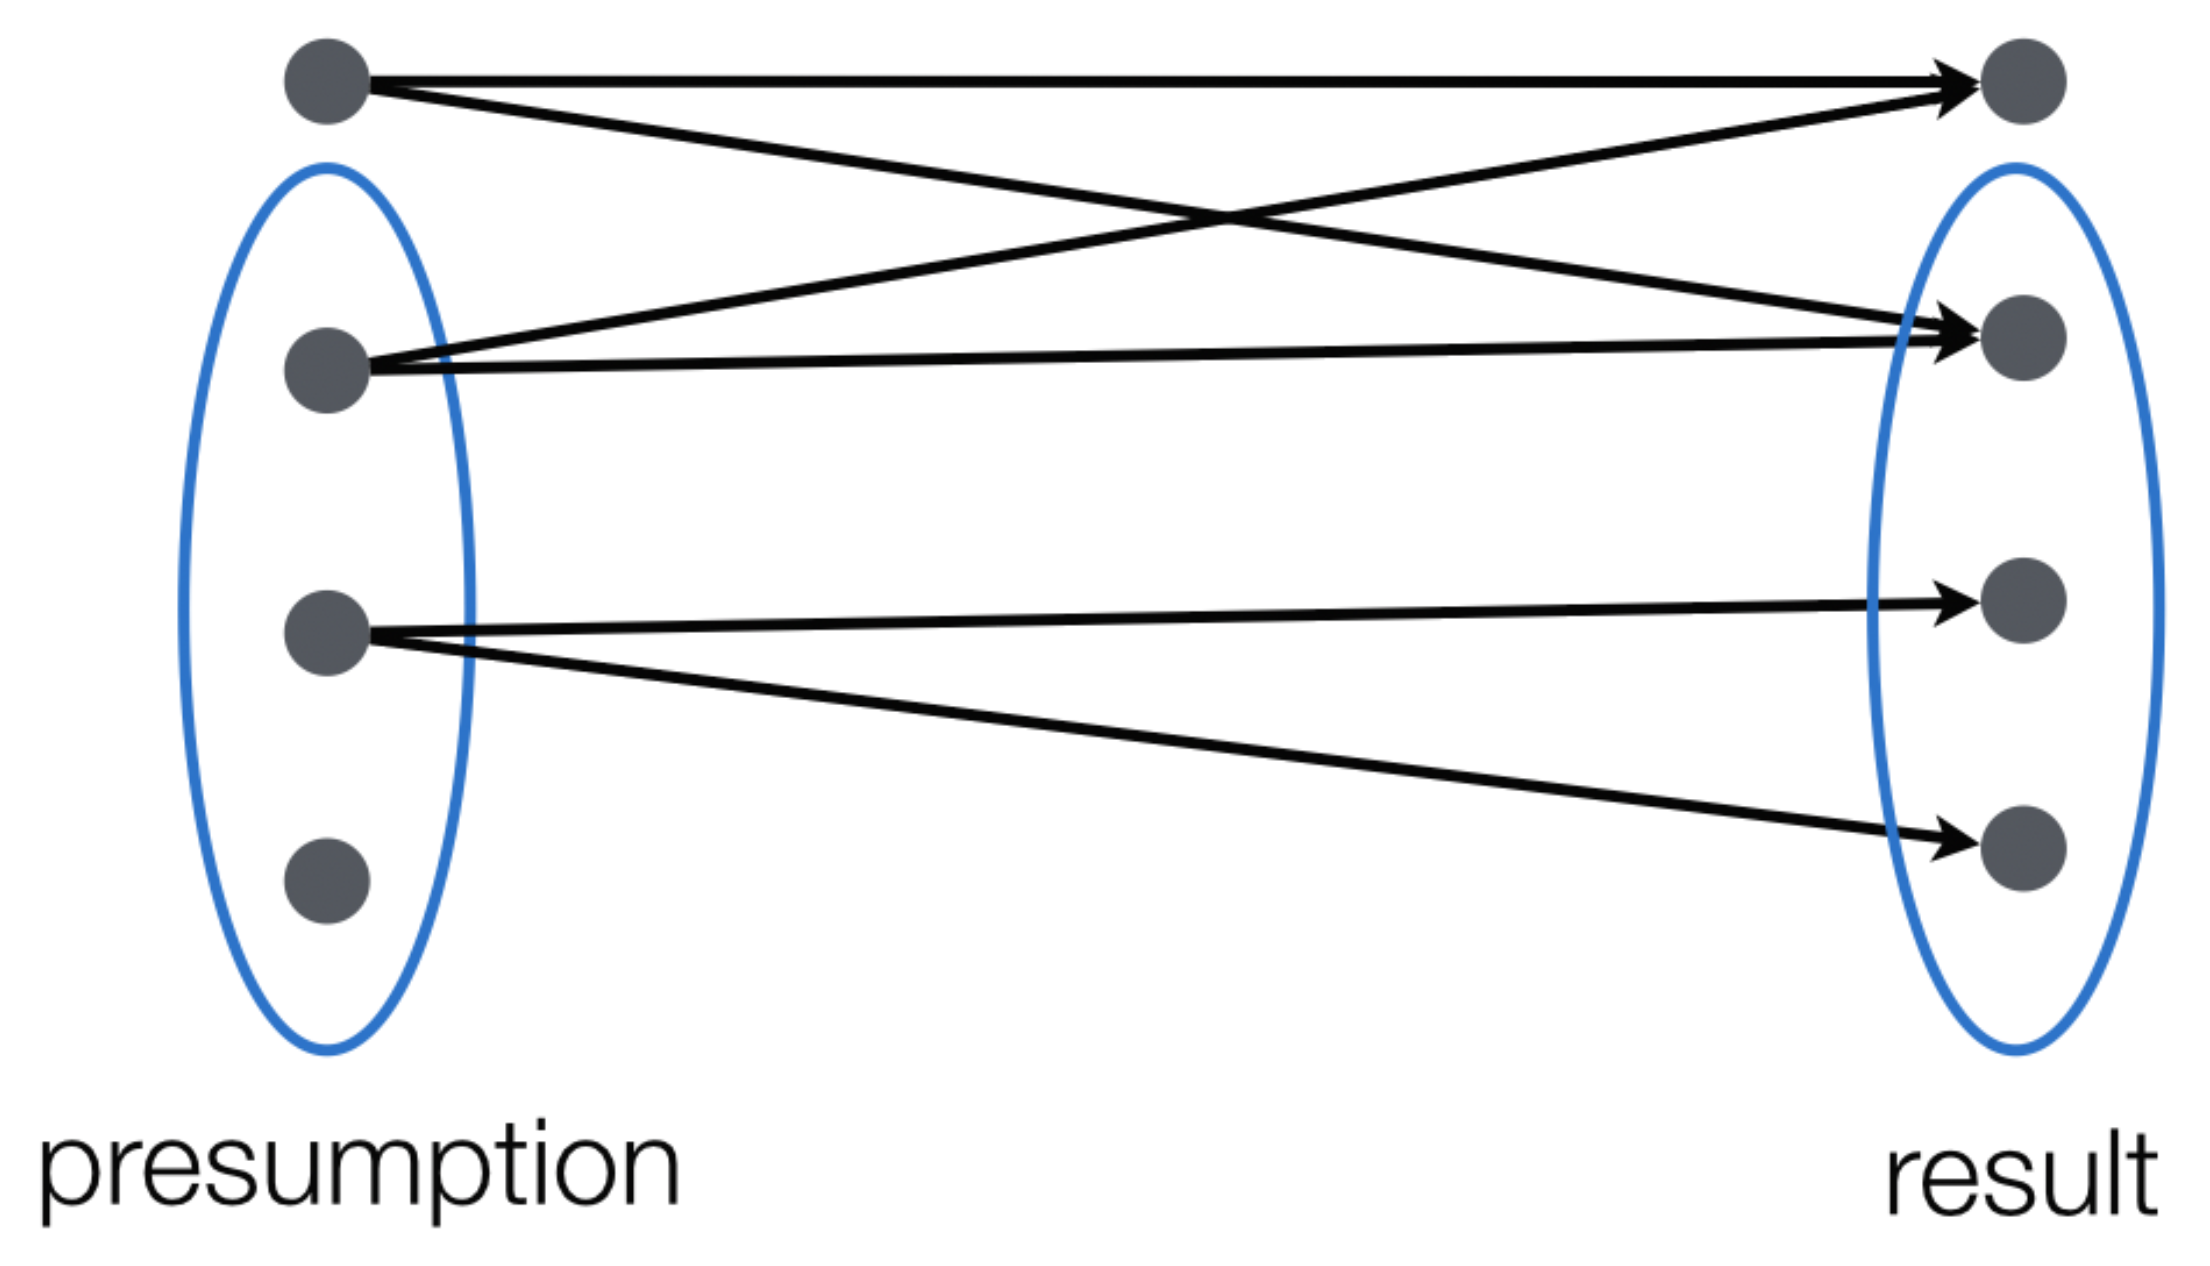
\includegraphics[width=\textwidth,height=0.5\textheight]{images/intro.png}
\caption{Source:
\href{https://dl.acm.org/doi/10.1145/3371078}{Incorrectness Logic
Paper}}
\end{figure}

\blockquote{\emph{Hoare triples speak the whole truth, where the under-approximate triples speak nothing but the truth.}}
\end{frame}

\section{A Unified Picture (Of Correctness and
Incorrectness)}\label{a-unified-picture-of-correctness-and-incorrectness}

\begin{frame}{Category-Theoretic Notion}
\phantomsection\label{category-theoretic-notion}
\begin{figure}
\centering
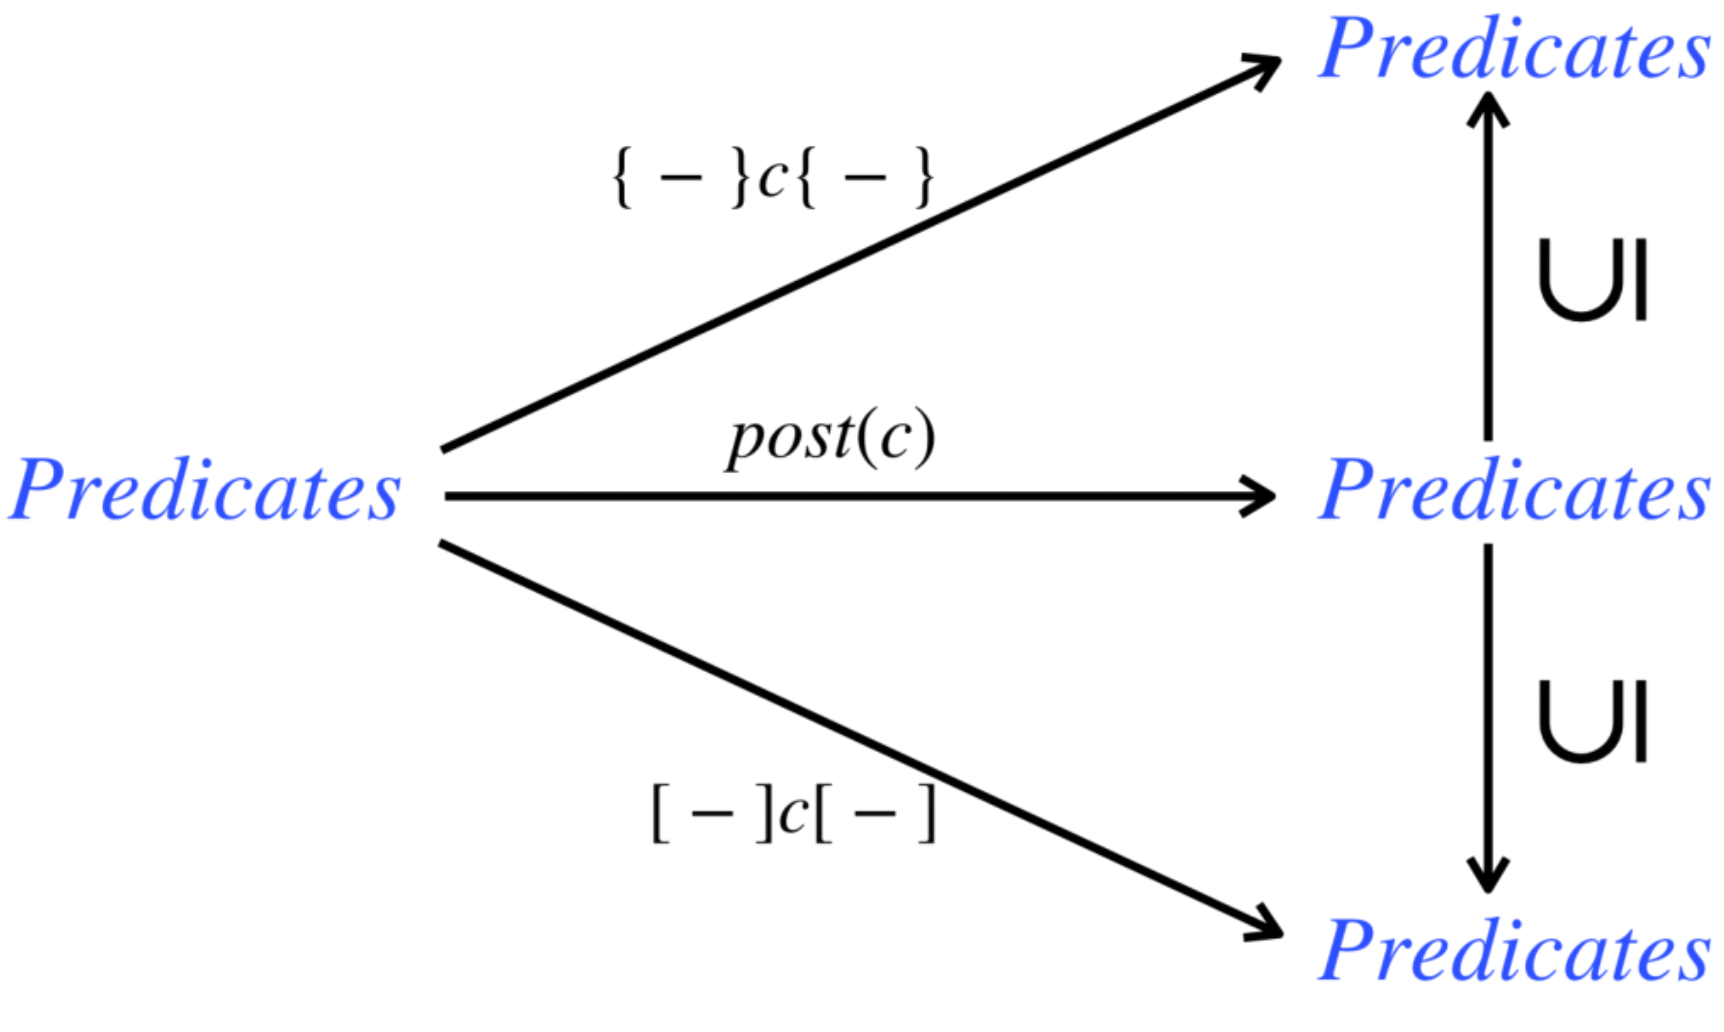
\includegraphics[width=\textwidth,height=0.4\textheight]{images/comm-diag.png}
\caption{Commuting Diagram (Source :
\href{https://dl.acm.org/doi/10.1145/3371078}{Incorrectness Logic
Paper})}
\end{figure}

\begin{itemize}
\item
  \textcolor{blue}{\emph{Predicates}}
  \(\approx 2^{\text{Program States}}\), arrows \(\approx\) binary
  relations on \textcolor{blue}{\emph{Predicates}}
\item
  \emph{post}(\(c\)) is a function, the other two are non-functional
\item
  \(\textcolor{blue}{[-]c[-]} = \text{\emph{post}}(c) ; \supseteq\) and
  \(\textcolor{red}{\{-\}c\{-\}} = \text{\emph{post}}(c) ; \subseteq\)
\item
  \emph{post}\((c)p\) = strongest post of \(p\) = weakest
  under-approximating post of \(p\)
\end{itemize}
\end{frame}

\begin{frame}{Reasoning Principles - I}
\phantomsection\label{reasoning-principles---i}
\begin{figure}
\centering
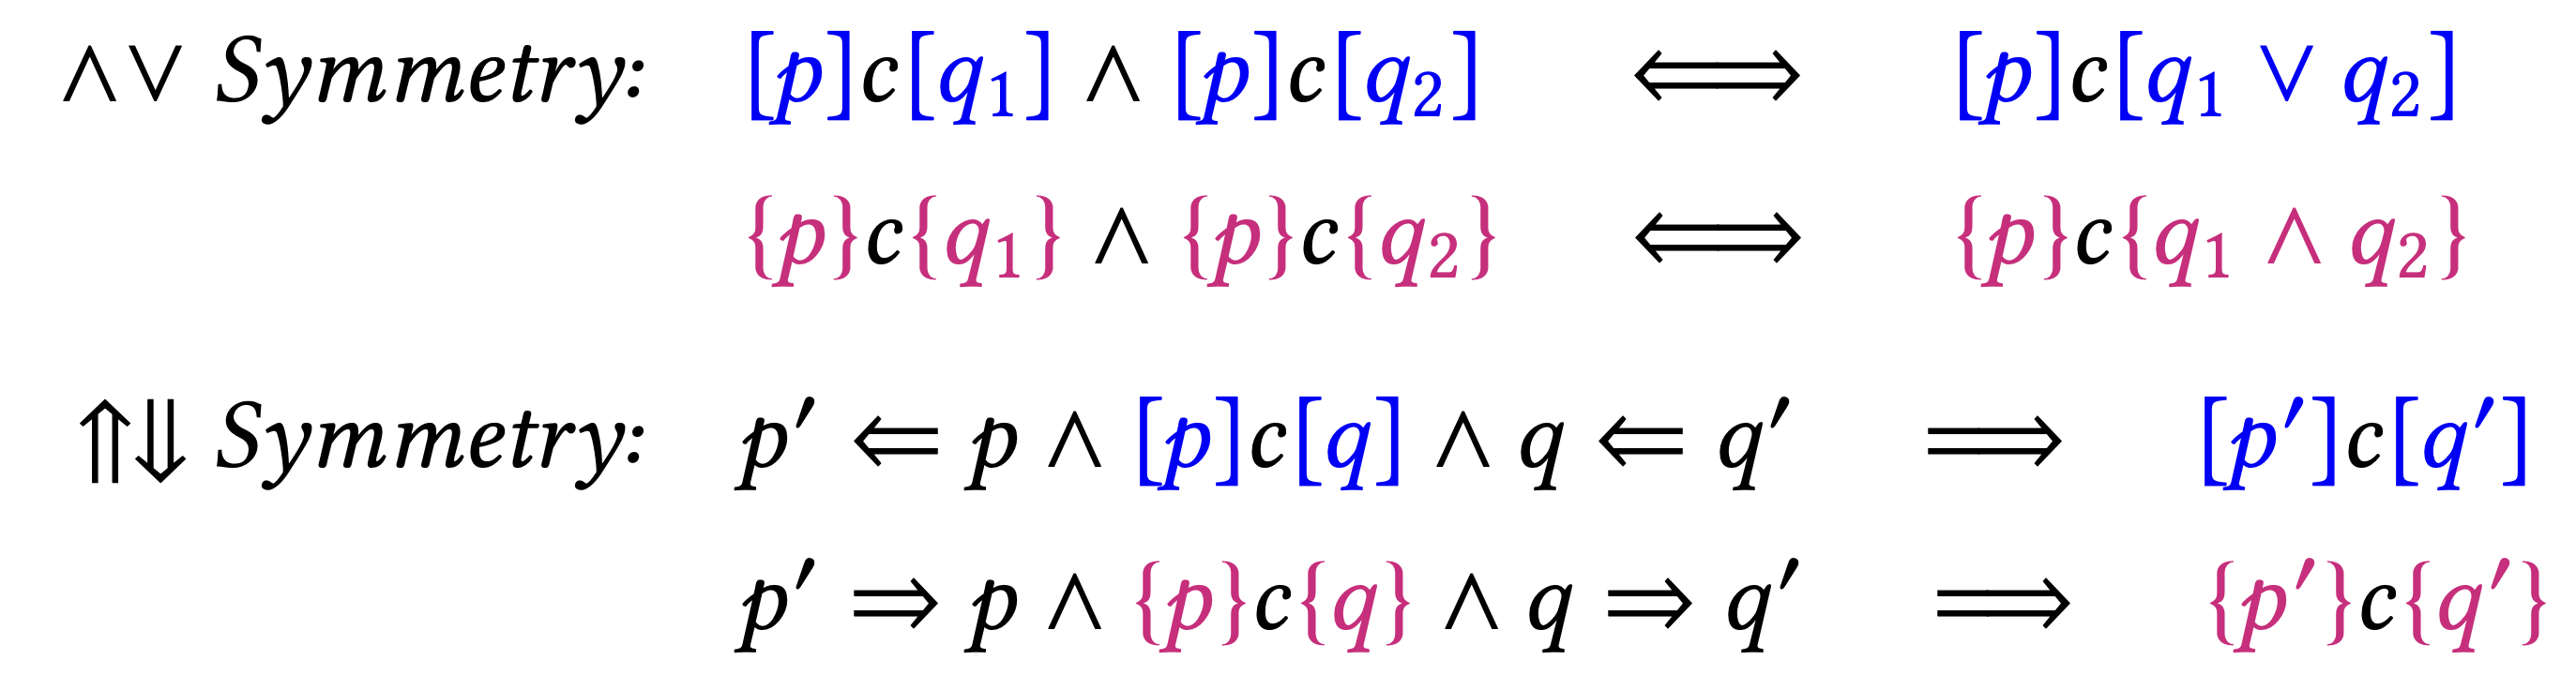
\includegraphics[width=\textwidth,height=0.4\textheight]{images/principles-1.png}
\caption{Correctness \& Incorrectness Principles (Source :
\href{https://dl.acm.org/doi/10.1145/3371078}{Incorrectness Logic
Paper})}
\end{figure}

\begin{itemize}
\tightlist
\item
  \(\blue{[p]c[q \lor r]} \implies \blue{[p]c[q]}\) allows you to
  \emph{drop paths} going forward.

  \begin{itemize}
  \tightlist
  \item
    Not possible in overapproximate logics - but can \emph{forget
    information} along each path
  \end{itemize}
\item
  Rules of consequence allow specifications to be adapted to broader
  contexts
\end{itemize}
\end{frame}

\begin{frame}{Reasoning Principles - II}
\phantomsection\label{reasoning-principles---ii}
\begin{figure}
\centering
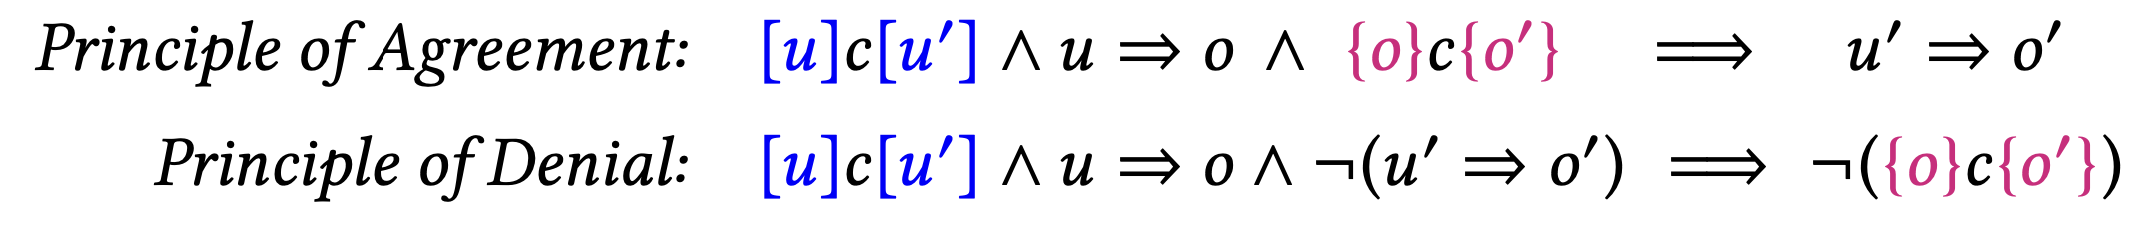
\includegraphics[width=\textwidth,height=0.2\textheight]{images/principles-2.png}
\caption{Correctness \& Incorrectness Principles (Source :
\href{https://dl.acm.org/doi/10.1145/3371078}{Incorrectness Logic
Paper})}
\end{figure}

\begin{figure}
\centering
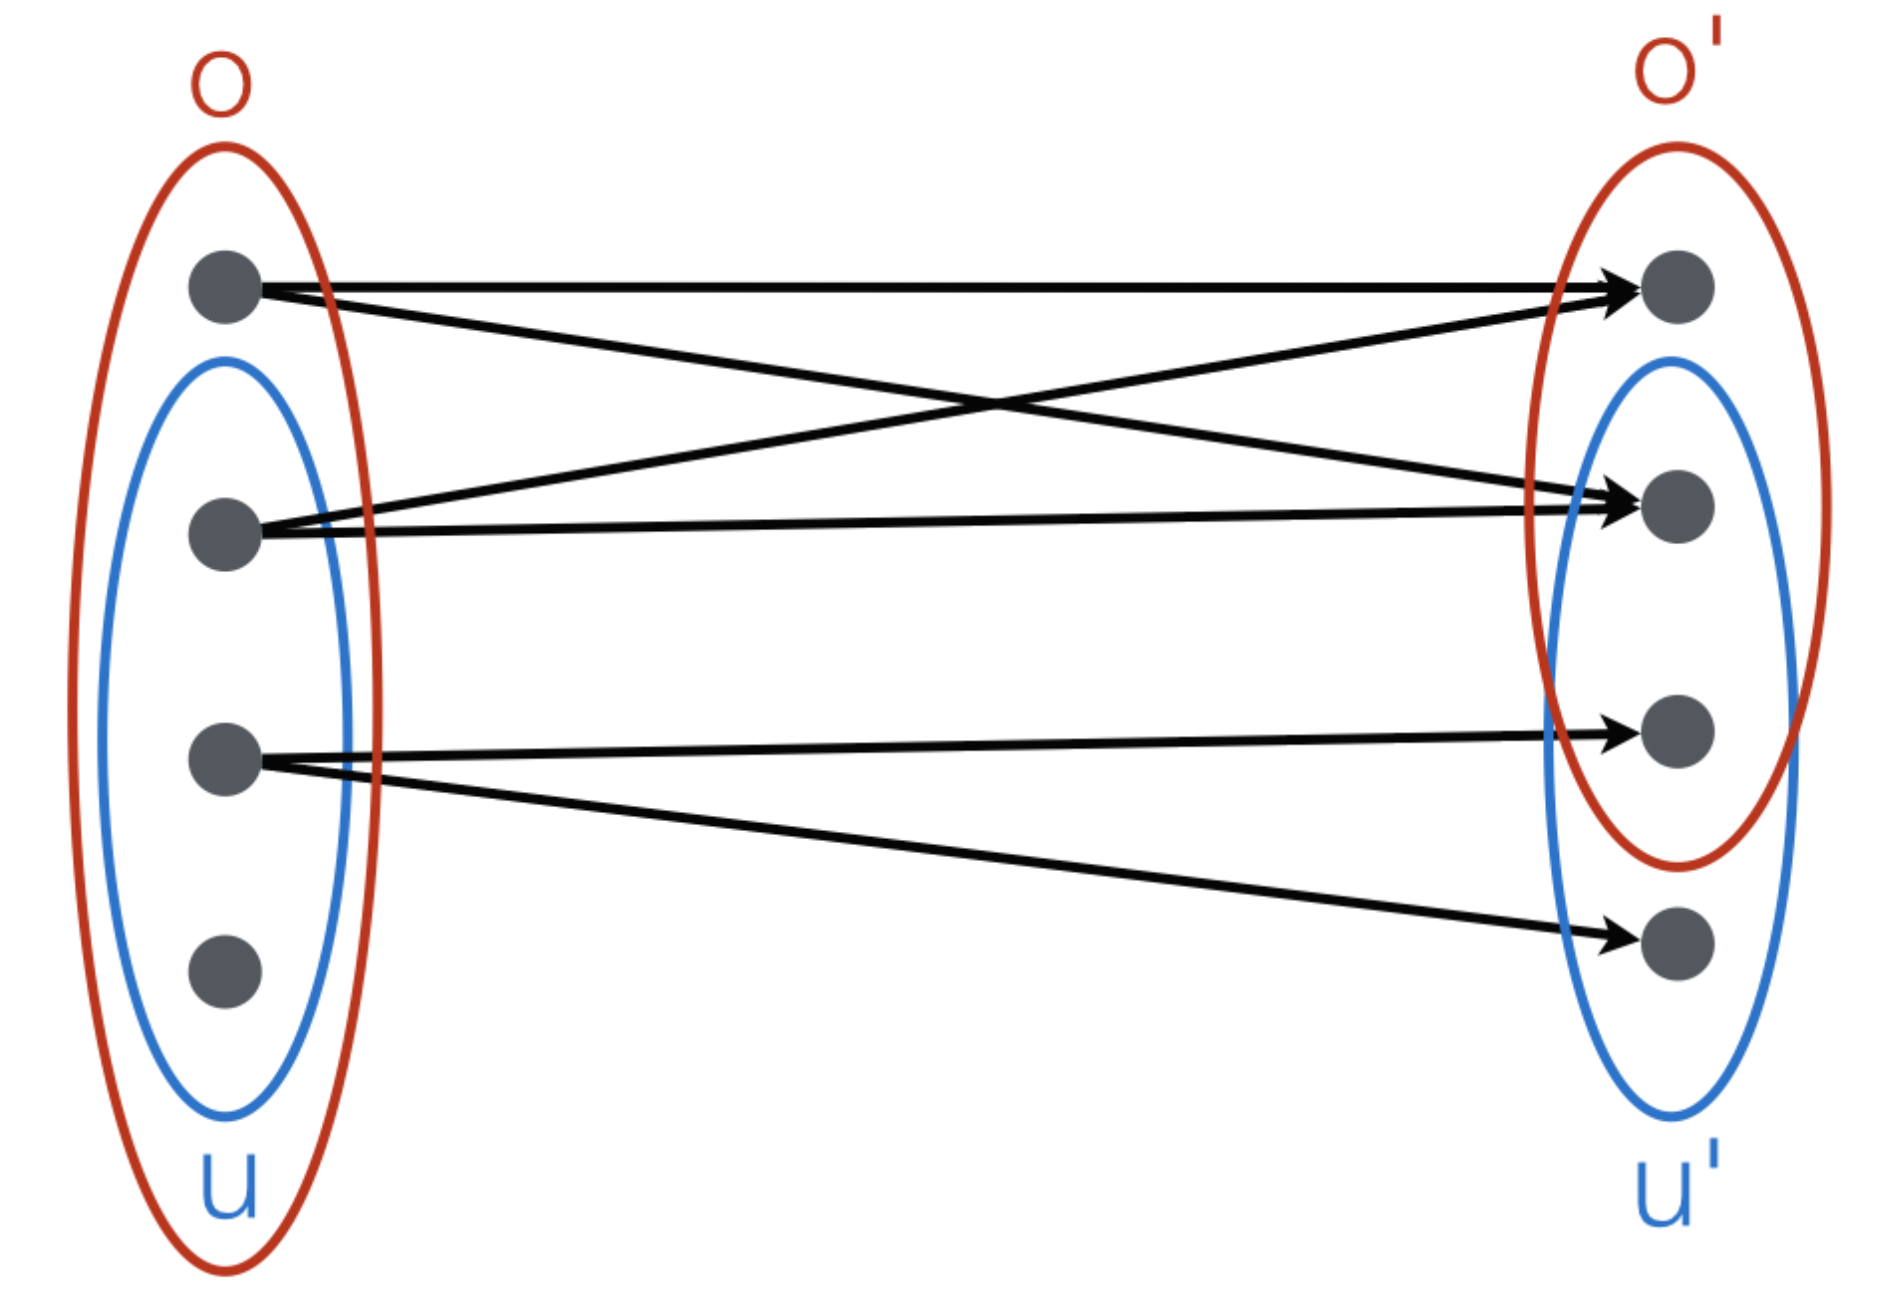
\includegraphics[width=\textwidth,height=0.3\textheight]{images/denial.png}
\caption{Analogy with Testing (Source :
\href{https://dl.acm.org/doi/10.1145/3371078}{Incorrectness Logic
Paper})}
\end{figure}

\begin{itemize}
\tightlist
\item
  Program testing works on the principle of denial (traditionally,
  \(|u| = |u'| = 1\), a test run)
\end{itemize}
\end{frame}

\begin{frame}{Isn't Incorrectness Just Not Correctness?}
\phantomsection\label{isnt-incorrectness-just-not-correctness}
\begin{itemize}
\item
  Yes, but we aren't powerful enough to precisely compute either!
\item
  \emph{'The inability to prove an over-approximate spec (whether found by a tool or specified by a human) does not imply an error in a program, and neither does not having found a bug imply that there are none: thus, the need for dedicated techniques for each.'}
\end{itemize}
\end{frame}

\section{Build Your Muscle}\label{build-your-muscle}

\begin{frame}[fragile]{Under-Approximating Triples - I}
\phantomsection\label{under-approximating-triples---i}
\[
\blue{[z = 11]}
\]

\begin{Shaded}
\begin{Highlighting}[]
\ControlFlowTok{if} \OperatorTok{(}\NormalTok{x is even}\OperatorTok{)} \OperatorTok{\{}
    \ControlFlowTok{if} \OperatorTok{(}\NormalTok{y is odd}\OperatorTok{)} \OperatorTok{\{}
\NormalTok{        z }\OperatorTok{=} \DecValTok{42}\OperatorTok{;}
    \OperatorTok{\}}
\OperatorTok{\}}
\end{Highlighting}
\end{Shaded}

\[
\blue{[z = 42]}
\]

\pause

This triple \emph{does not hold}! The state
\texttt{{[}z\ :\ 42,\ x\ :\ 1,\ y\ :\ 3{]}} has no predecessor!
\end{frame}

\begin{frame}[fragile]{Under-Approximating Triples - II}
\phantomsection\label{under-approximating-triples---ii}
\[
\blue{[true]}
\]

\begin{Shaded}
\begin{Highlighting}[]
\ControlFlowTok{if} \OperatorTok{(}\NormalTok{x is even}\OperatorTok{)} \OperatorTok{\{}
    \ControlFlowTok{if} \OperatorTok{(}\NormalTok{y is odd}\OperatorTok{)} \OperatorTok{\{}
\NormalTok{        z }\OperatorTok{=} \DecValTok{42}\OperatorTok{;}
    \OperatorTok{\}}
\OperatorTok{\}}
\end{Highlighting}
\end{Shaded}

\[
\blue{[z = 42]}
\]

\pause

This triple \emph{holds}!
\end{frame}

\begin{frame}[fragile]{Under-Approximating Triples - III}
\phantomsection\label{under-approximating-triples---iii}
\[
\blue{[z = 11]}
\]

\begin{Shaded}
\begin{Highlighting}[]
\ControlFlowTok{if} \OperatorTok{(}\NormalTok{x is even}\OperatorTok{)} \OperatorTok{\{}
    \ControlFlowTok{if} \OperatorTok{(}\NormalTok{y is odd}\OperatorTok{)} \OperatorTok{\{}
\NormalTok{        z }\OperatorTok{=} \DecValTok{42}\OperatorTok{;}
    \OperatorTok{\}}
\OperatorTok{\}}
\end{Highlighting}
\end{Shaded}

\[
\blue{[z = 42 \land (x \text{ is even }) \land (y \text{ is odd })]}
\]

\pause

This triple \emph{holds}!
\end{frame}

\begin{frame}[fragile]{Under-Approximating Triples - IV}
\phantomsection\label{under-approximating-triples---iv}
\[
\blue{[\true]}
\]

\begin{Shaded}
\begin{Highlighting}[]
\ControlFlowTok{if} \OperatorTok{(}\NormalTok{x is even}\OperatorTok{)} \OperatorTok{\{}
    \ControlFlowTok{if} \OperatorTok{(}\NormalTok{y is odd}\OperatorTok{)} \OperatorTok{\{}
\NormalTok{        z }\OperatorTok{=} \DecValTok{42}\OperatorTok{;}
    \OperatorTok{\}}
\OperatorTok{\}}
\end{Highlighting}
\end{Shaded}

\[
\blue{[z = 42 \land (x \text{ is even }) \land (y \text{ is odd })]}
\]

\pause

This triple \emph{holds}!
\end{frame}

\begin{frame}[fragile]{Specifying Incorrectness}
\phantomsection\label{specifying-incorrectness}
\begin{itemize}
\tightlist
\item
  Reasoning about errors?
\end{itemize}

\pause

\begin{itemize}
\tightlist
\item
  Have separate result-assertion forms for normal and (erroneous or
  abnormal) termination.
\end{itemize}

\begin{Shaded}
\begin{Highlighting}[]
\DataTypeTok{void}\NormalTok{ foo}\OperatorTok{(}\DataTypeTok{char} \OperatorTok{*}\NormalTok{ str}\OperatorTok{)}
\CommentTok{/* presumes: [ *str[]==s ]}
\CommentTok{   achieves: [ er: *str[]==s \&\& length(s) \textgreater{} 16 ] */}
\OperatorTok{\{}
    \DataTypeTok{char}\NormalTok{ buf}\OperatorTok{[}\DecValTok{16}\OperatorTok{];}
\NormalTok{    strcpy}\OperatorTok{(}\NormalTok{buf}\OperatorTok{,}\NormalTok{str}\OperatorTok{);}
\OperatorTok{\}}

\DataTypeTok{int}\NormalTok{ main}\OperatorTok{(}\DataTypeTok{int}\NormalTok{ argc}\OperatorTok{,} \DataTypeTok{char} \OperatorTok{*}\NormalTok{argv}\OperatorTok{[])}
\OperatorTok{\{}\NormalTok{ foo}\OperatorTok{(}\NormalTok{argv}\OperatorTok{[}\DecValTok{1}\OperatorTok{]);} \OperatorTok{\}}
\end{Highlighting}
\end{Shaded}

\begin{itemize}
\tightlist
\item
  Spec: if the length of the input string is greater than 16 then we can
  get an error (in this case a buffer overflow).
\end{itemize}
\end{frame}

\begin{frame}[fragile]{Under-approximate Success}
\phantomsection\label{under-approximate-success}
\begin{itemize}
\tightlist
\item
  Why not over-approximate for successful and under-approximate for
  erroneous termination?

  \begin{itemize}
  \tightlist
  \item
    Under-approximate result assertions describing successful
    computations can help us \textbf{soundly discover bugs that come
    after a procedure is called}.
  \end{itemize}
\end{itemize}

\pause

\begin{Shaded}
\begin{Highlighting}[]
\DataTypeTok{void}\NormalTok{ mkeven}\OperatorTok{()}
\CommentTok{/* presumes: [true], wrong achieves: [ok: x==2 || x==4] */}
\OperatorTok{\{}\NormalTok{ x}\OperatorTok{=}\DecValTok{2}\OperatorTok{;} \OperatorTok{\}}

\DataTypeTok{void}\NormalTok{ usemkeven}\OperatorTok{()}
\OperatorTok{\{}\NormalTok{ mkeven}\OperatorTok{();} \ControlFlowTok{if} \OperatorTok{(}\NormalTok{x}\OperatorTok{==}\DecValTok{4}\OperatorTok{)} \OperatorTok{\{}\NormalTok{error}\OperatorTok{();\}} \OperatorTok{\}}
\end{Highlighting}
\end{Shaded}

\begin{itemize}
\tightlist
\item
  We don't want false positives!
\end{itemize}
\end{frame}

\section{Proof System}\label{proof-system}

\begin{frame}[fragile]{Setup}
\phantomsection\label{setup}
\begin{itemize}
\item
  Simple imperative language. \texttt{error()} halts execution and
  raises an error signal, \texttt{er}.
\item
  Abnormal control flows impact reasoning about sequential composition

  \begin{itemize}
  \tightlist
  \item
    Solution: associate assertions with a set of exit conditions
    \(\epsilon\)
  \item
    \(\epsilon\) includes (at least) \(\ok\) for normal termination and
    \(\er\) causes by \texttt{error()}
  \end{itemize}
\item
  \(\blue{[p]} C \blue{[\epsilon : q]}\) = \(q\) under-approximates the
  states when \(C\) exits via \(\epsilon\) starting from states in
  \(p\).
\item
  \(x\) is \textbf{not} free in \(p\) iff
  \(\sigma \in p \iff (\forall v \,.\, (\sigma | x \mapsto v) \in p)\).
  \red{[BUG]}
\item
  Treat \(p,q\) semantically (i.e., any \(\subseteq \Sigma\), the set of
  program states) -- don't fix a language.

  \begin{itemize}
  \tightlist
  \item
    By treating assertions semantically, we are essentially appealing to
    mathematics (or set theory) as an oracle in our proof theory when we
    use \(\simplies\) in proof rules.
  \end{itemize}
\item
  \(\blue{[p]} C \green{[\ok : q]} \red{[\er : r]}\) as shorthand for
  \(\blue{[p]} C \green{[\ok : q]}\) and
  \(\blue{[p]} C \red{[\er : r]}\).
\end{itemize}
\end{frame}

\begin{frame}{Generic Proof Rules - I}
\phantomsection\label{generic-proof-rules---i}
\begin{figure}
\centering
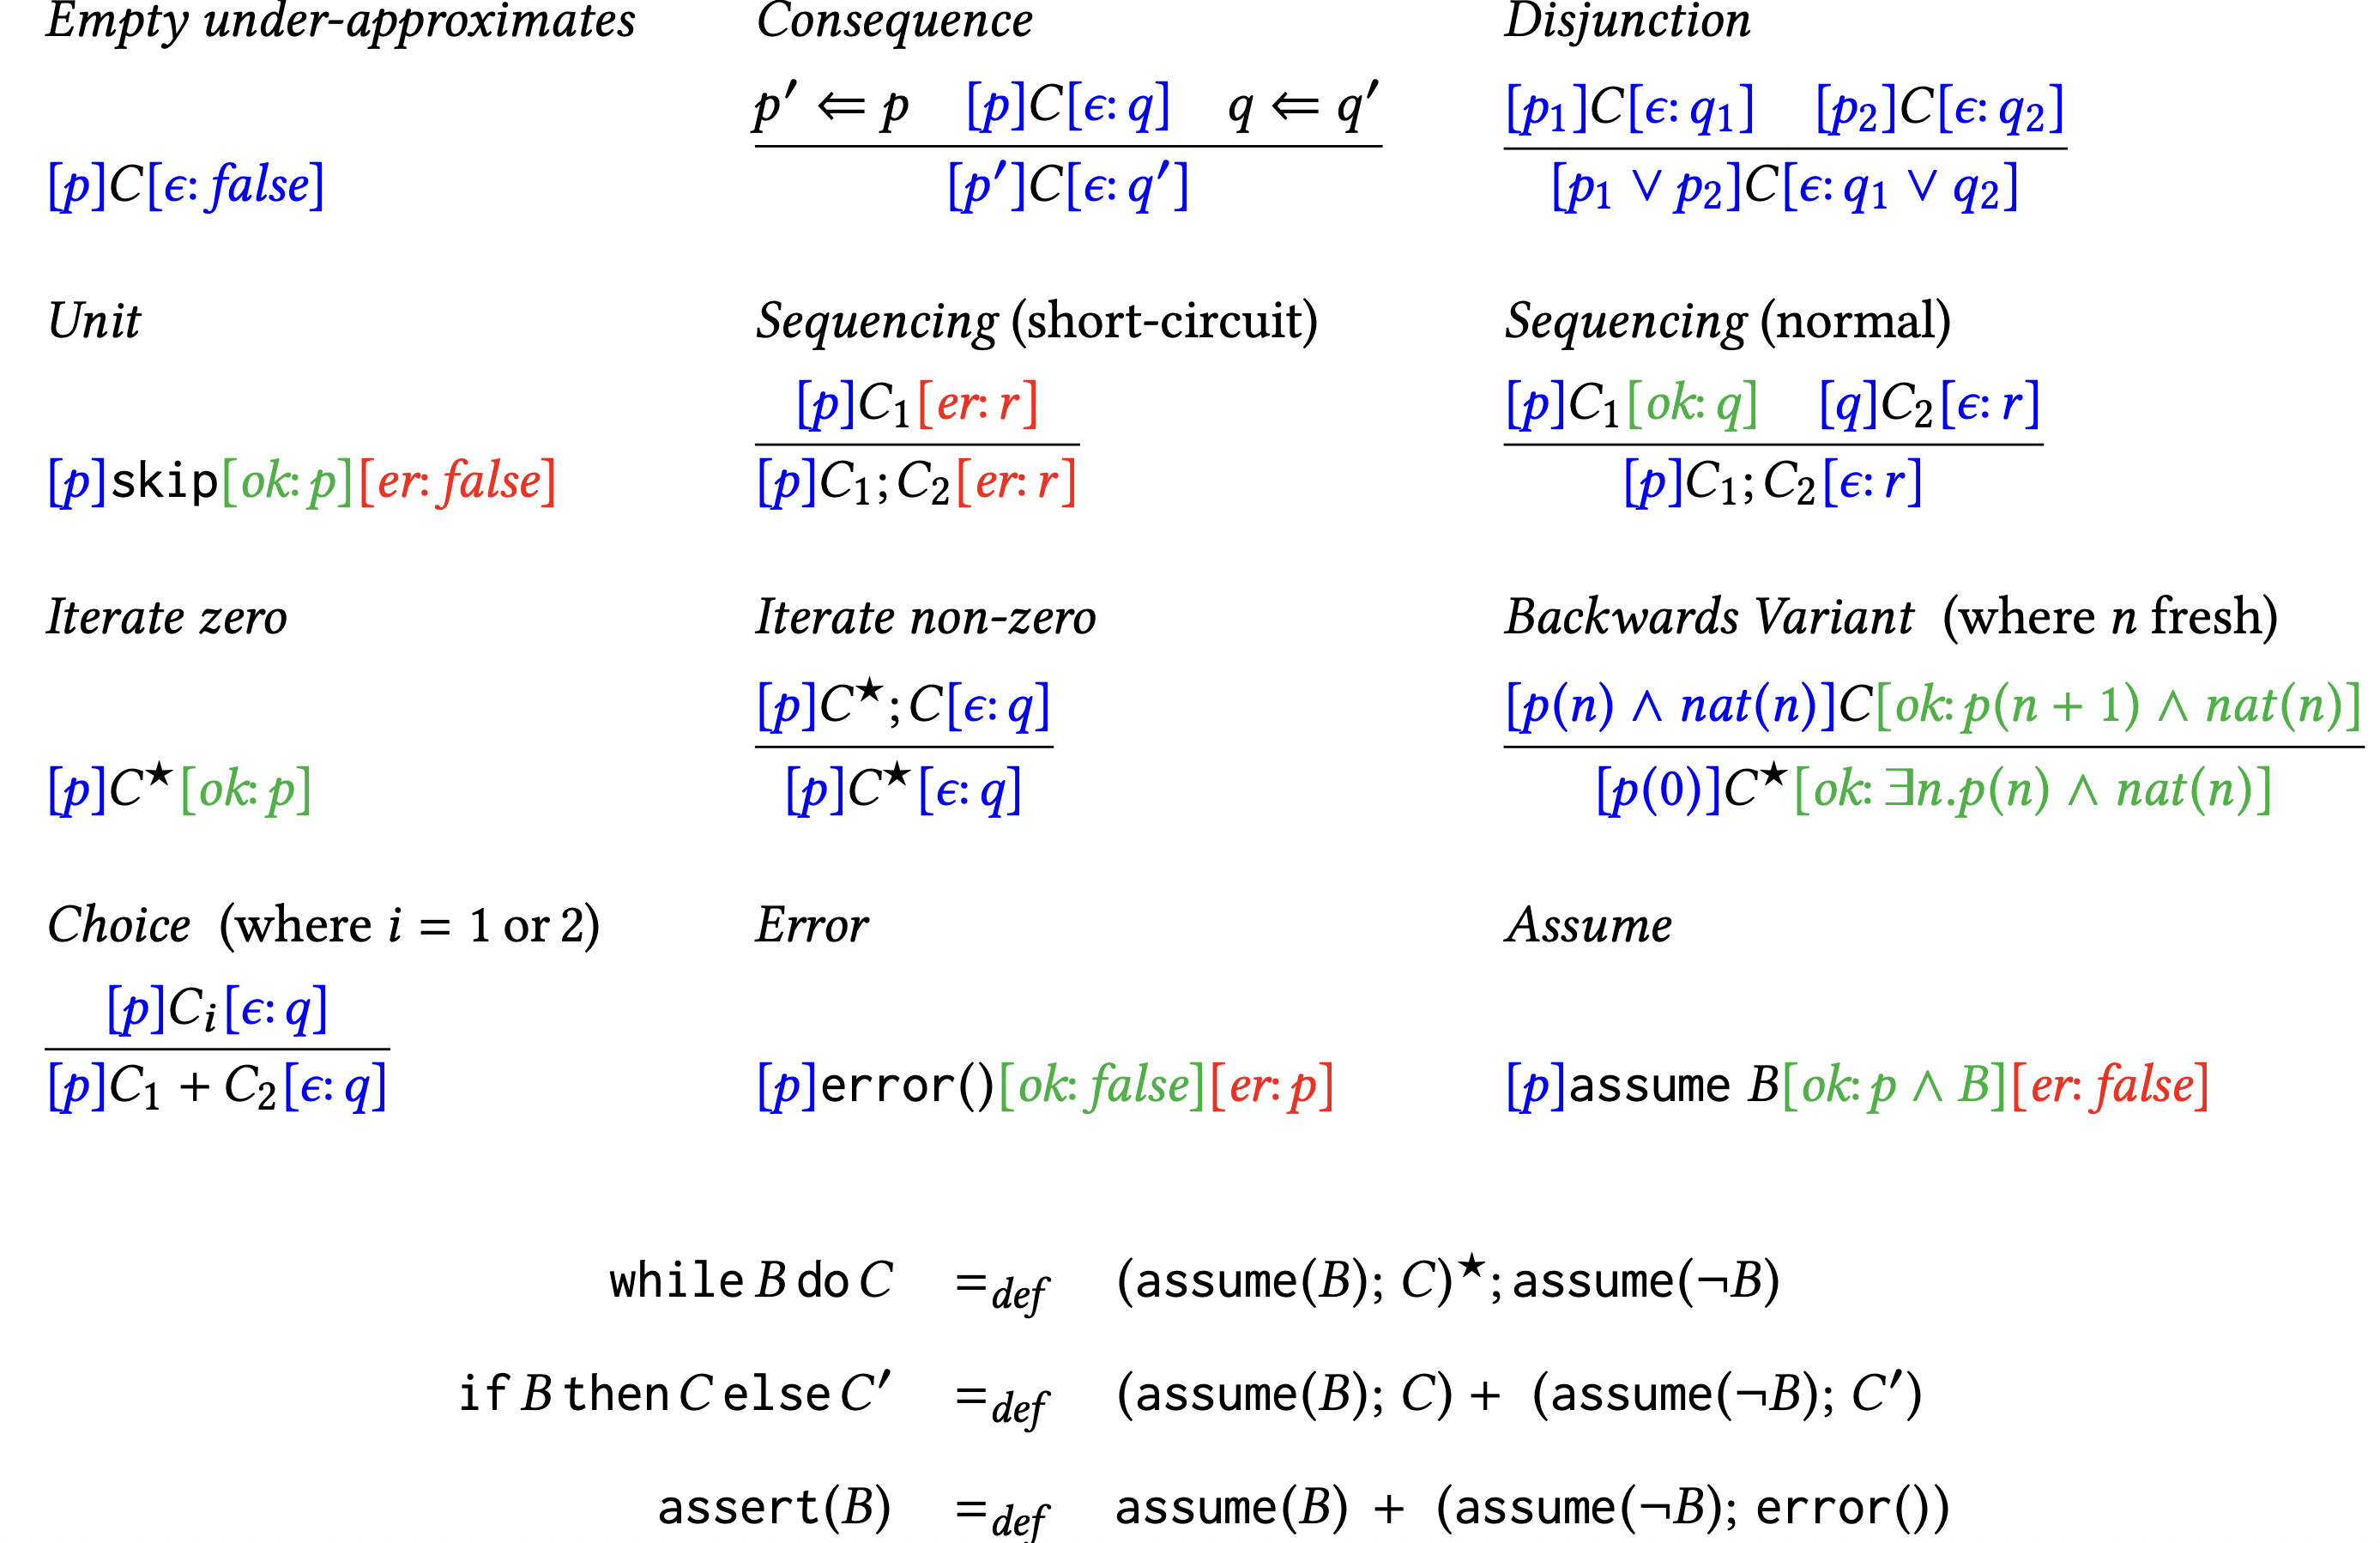
\includegraphics{images/generic.png}
\caption{Generic Proof Rules of Incorrectness Logic (Source:
\href{https://dl.acm.org/doi/10.1145/3371078}{Incorrectness Logic
Paper})}
\end{figure}
\end{frame}

\begin{frame}[fragile]{Generic Proof Rules - Axioms}
\phantomsection\label{generic-proof-rules---axioms}
\begin{itemize}
\tightlist
\item
  Valid across different models of states and commands

  \begin{itemize}
  \tightlist
  \item
    Usual: States = \(\Vars \to \Vals\) and Commands = Binary Relations
    on States
  \item
    Others based on traces, separation logic etc.
  \end{itemize}
\end{itemize}

\begin{center}
\begin{tabular}{cc}
\inference[Assume]{}{\blue{[p]} \Assume B \green{[\ok : p \land B]} \red{[\er : \false]}} &
\inference[Skip]{}{\blue{[p]} \Skip \green{[\ok : p]} \red{[\er : \false]}} \\ \\
\inference[Empty under-approximates]{}{\blue{[p]} C \blue{[\epsilon:\false]}} &
\end{tabular}
\end{center}

\begin{itemize}
\item
  \texttt{assume(B)} statement : \texttt{B} is a Boolean expression, can
  be from an otherwise-unspecified first-order logic signature.
\item
  Axioms for \texttt{assume} and \texttt{skip} : give the expected
  assertions for normal termination, but specify \texttt{false} (the
  empty set of states) for abnormal.
\end{itemize}
\end{frame}

\begin{frame}{Generic Proof Rules - Consequence, Disjunction \& Choice}
\phantomsection\label{generic-proof-rules---consequence-disjunction-choice}
\begin{center}
\begin{tabular}{c}
\inference[Consequence]{p' \simpliedby p \quad \blue{[p]} C \blue{[\epsilon:q]} \quad q \simpliedby q'}{\blue{[p']} C \blue{[\epsilon:q']}} \\ \\
\inference[Disjunction]{
    \ruleeps{p_1}{C}{q_1} \quad \ruleeps{p_2}{C}{q_2}
}{
    \ruleeps{p_1 \lor p_2}{C}{q_1 \lor q_2}
} \\ \\
\inference[Choice (where $i=1,2$)]{ \ruleeps{p}{C_i}{q} }{ \ruleeps{p}{C_1 + C_2}{q} }
\end{tabular}
\end{center}

\begin{itemize}
\tightlist
\item
  The rule of consequence lets us \emph{enlarge (weaken) the pre} and
  \emph{shrink (strengthen) the post-assertion}.

  \begin{itemize}
  \tightlist
  \item
    Allows us to \emph{drop disjuncts in the post} and \emph{drop
    conjuncts in the pre}.
  \end{itemize}
\item
  \emph{`Enlarging the pre was used in the Abductor tool
  (\href{https://www.researchgate.net/publication/220431326_Compositional_Shape_Analysis_by_Means_of_Bi-Abduction}{{[}Calcagno
  et al.~2011{]}}, which led to Facebook Infer), when guessing
  pre-conditions in programs with loops.'}

  \begin{itemize}
  \tightlist
  \item
    Was unsound in the over-approximating logic used there, required a
    re-execution step which filtered out unsound pre-conditions
  \end{itemize}
\end{itemize}
\end{frame}

\begin{frame}{Generic Proof Rules - Sequencing and Iteration}
\phantomsection\label{generic-proof-rules---sequencing-and-iteration}
\begin{center}
\begin{tabular}{cc}
    \emph{Sequencing(short-circuit)} & \emph{Sequencing(normal)} \\ & \\
    \inference[]{
        \ruleer{p}{C_1}{r}
    }{
        \ruleer{p}{C_1;C_2}{r}
    } &
    \inference[]{
        \ruleok{p}{C_1}{q} \quad
        \ruleeps{q}{C_2}{r}
    }{
        \ruleeps{p}{C_1;C_2}{r}
    } \\ & \\
    \emph{Iterate zero} & \emph{Iterate non-zero} \\ & \\
    \inference[]{}{
        \ruleok{p}{C^{*}}{p}
    } &
    \inference[]{
        \ruleeps{p}{C^{*} ; C}{q}
    }{
        \ruleeps{p}{C^{*}}{q}
    }
\end{tabular}
\end{center}

\begin{itemize}
\tightlist
\item
  The \emph{Iterate zero} rule shows that \textbf{any assertion is a
  valid under-approximate invariant for Kleene iteration}.

  \begin{itemize}
  \tightlist
  \item
    Loop invariants don't play a central role in under-approximate
    reasoning. Notion of \emph{subvariants} mentioned in
    \href{http://www0.cs.ucl.ac.uk/staff/p.ohearn/papers/POPL23TutorialSemanticsPart.pdf}{POPL'23
    tutorial}.
  \end{itemize}
\item
  The \emph{Iterate non-zero} rule uses \(C^{*} ; C\) rather than
  \(C ; C^{*}\) to help reasoning about cases where an error is thrown
  inside an iteration. Will see an example later.
\end{itemize}
\end{frame}

\begin{frame}{Generic Proof Rules - Derived Choice and Iteration,
Backwards Variant}
\phantomsection\label{generic-proof-rules---derived-choice-and-iteration-backwards-variant}
\begin{center}
\begin{tabular}{cc}
    \emph{Derived Unrolling Rule} & \emph{Derived Rule of Choice} \\ & \\
    \inference[]{
    \ruleeps{p}{C^i}{q_i} \,,\, \text{ all } i \leq \text{ bound }
}{
    \ruleeps{p}{C^{*}}{ \bigvee_{i \leq \text{bound}} q_i }
} &
    \inference[]{
    \ruleeps{p}{C_1}{q_1} \quad \ruleeps{p}{C_2}{q_2}
}{
    \ruleeps{p}{C_1 + C_2}{q_1 \lor q_2}
}
\end{tabular}
\end{center}

\begin{itemize}
\item
  One of the things that iteration can do is execute its body \(i\)
  times.
\item
  The \emph{Unrolling} rule gives a similar capability symbolic bounded
  model checking (but we need the \emph{Backwards Variant} rule too in
  general).
\end{itemize}

\begin{center}
\begin{tabular}{c}
    \inference[Backwards Variant (where $n$ fresh)]{
    \ruleeps{ p(n) \land \Nat(n) }{C}{ p(n+1) \land \Nat(n) }
}{
    \ruleeps{ p(0) }{C^{*}}{ \exists n \,.\, p(n) \land \Nat(n) }
}
\end{tabular}
\end{center}

\begin{itemize}
\tightlist
\item
  \(p(.)\) = a parameterized predicate (a function from expressions to
  predicates).
\end{itemize}
\end{frame}

\begin{frame}{Backwards Variant relation with Program Termination}
\phantomsection\label{backwards-variant-relation-with-program-termination}
\begin{itemize}
\tightlist
\item
  \(\ruleeps{\text{presumption}}{c}{\text{result}}\) expresses a
  reachability property that involves termination.

  \begin{itemize}
  \tightlist
  \item
    \emph{Every state in the result is reachable from some state in the
    presumption.}
  \end{itemize}
\item
  But this does not imply that a loop must terminate on all executions!

  \begin{itemize}
  \tightlist
  \item
    Enough paths terminate to cover all the states in result, while
    other paths may diverge.
  \end{itemize}
\item
  \emph{Backward variant} rule is similar to proof rules for proving
  program termination (typically use a ``variant'' that decreases on
  each loop iteration)

  \begin{itemize}
  \tightlist
  \item
    But reflects the \emph{backward} nature of this property. \(p\) goes
    down when executing backwards.
  \end{itemize}
\item
  What about the forward variant?
  \(\ruleok{\exists n \,.\, p(n) \land \Nat(n)}{C^{*}}{p(0)}\).
\end{itemize}

\pause

\begin{itemize}
\tightlist
\item
  It is always true :)
\end{itemize}
\end{frame}

\begin{frame}{Reachability and Liveness}
\phantomsection\label{reachability-and-liveness}
\begin{itemize}
\item
  Liveness : ``something (good) will eventually happen''.
\item
  Our reachability property:

  \begin{itemize}
  \item
    Backwards: For every state in the result, it is possible to
    eventually reach a state in the pre by executing backwards.
  \item
    Forwards: If we \emph{explore (enumerate pre-states, backtrack,
    dovetail)} executions from all pre-states, then eventually any given
    state in the result will be encountered.
  \end{itemize}
\item
  The ``eventually'' in our forwards does not concern all paths, rather
  it is an ``existential liveness property''.
\item
  The over-approximating triple
  \(\red{\{\text{pre}\}}C\red{\{\text{post}\}}\) describes a safety
  property, that ``nothing bad (= not post) will happen''.
\end{itemize}
\end{frame}

\begin{frame}[fragile]{Specific Proof Rules - Variables and Mutation}
\phantomsection\label{specific-proof-rules---variables-and-mutation}
\begin{figure}
\centering
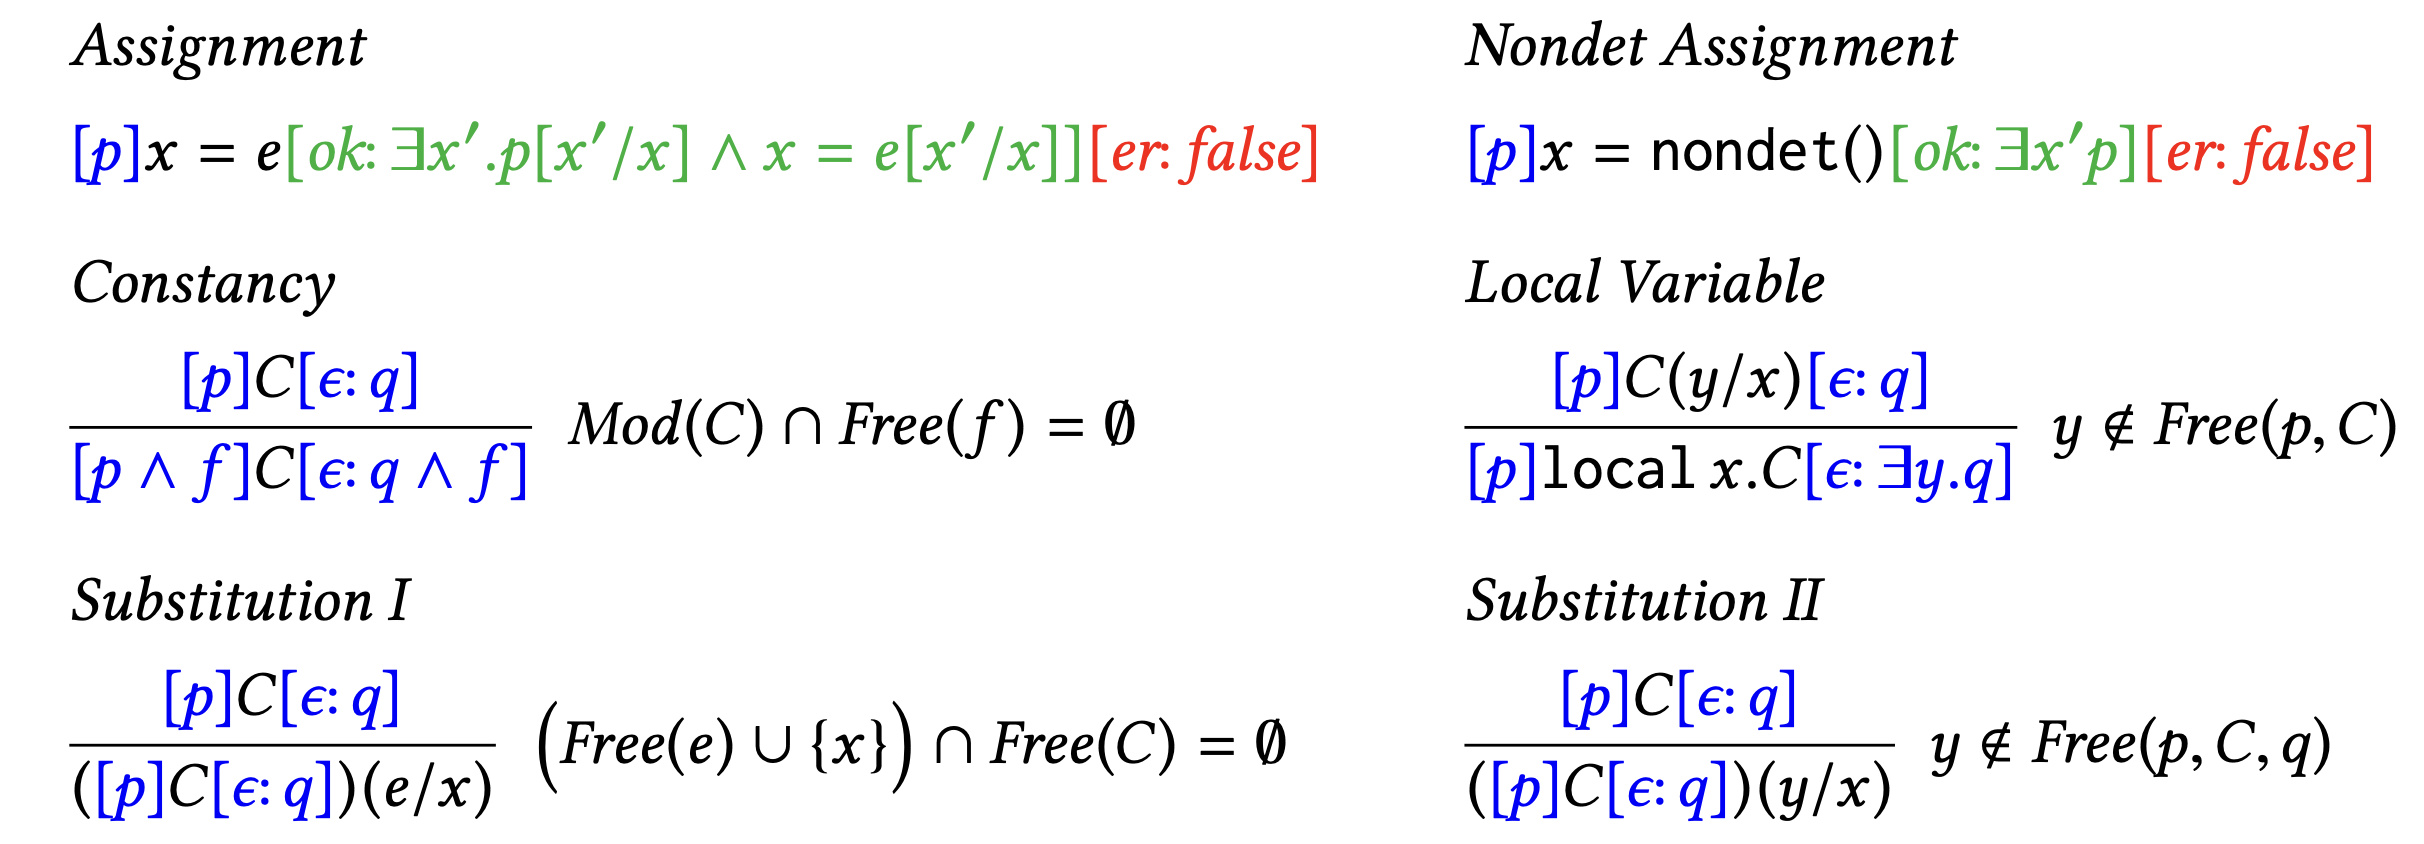
\includegraphics[width=\textwidth,height=0.3\textheight]{images/specific.png}
\caption{Rules for Variables and Mutation (Source:
\href{https://dl.acm.org/doi/10.1145/3371078}{Incorrectness Logic
Paper})}
\end{figure}

\begin{itemize}
\item
  Sound when states are functions of type \(\Vars \to \Vals\).
\item
  \emph{Mod}\((C)\) is the set of variables modified by assignment
  statements in \(C\), and \emph{Free}\((r)\) is the set of free
  variables in an assertion \(r\).
\item
  \texttt{e} and \texttt{nondet()} are syntactically distinct.

  \begin{itemize}
  \tightlist
  \item
    \texttt{e} is an expression built up from a first-order logic
    signature, can appear within assertions, and is side-effect free.
  \item
    \texttt{nondet()} does not appear in assertions.
  \end{itemize}
\end{itemize}
\end{frame}

\begin{frame}[fragile]{Specific Proof Rules - Variables and Mutation}
\phantomsection\label{specific-proof-rules---variables-and-mutation-1}
\begin{figure}
\centering
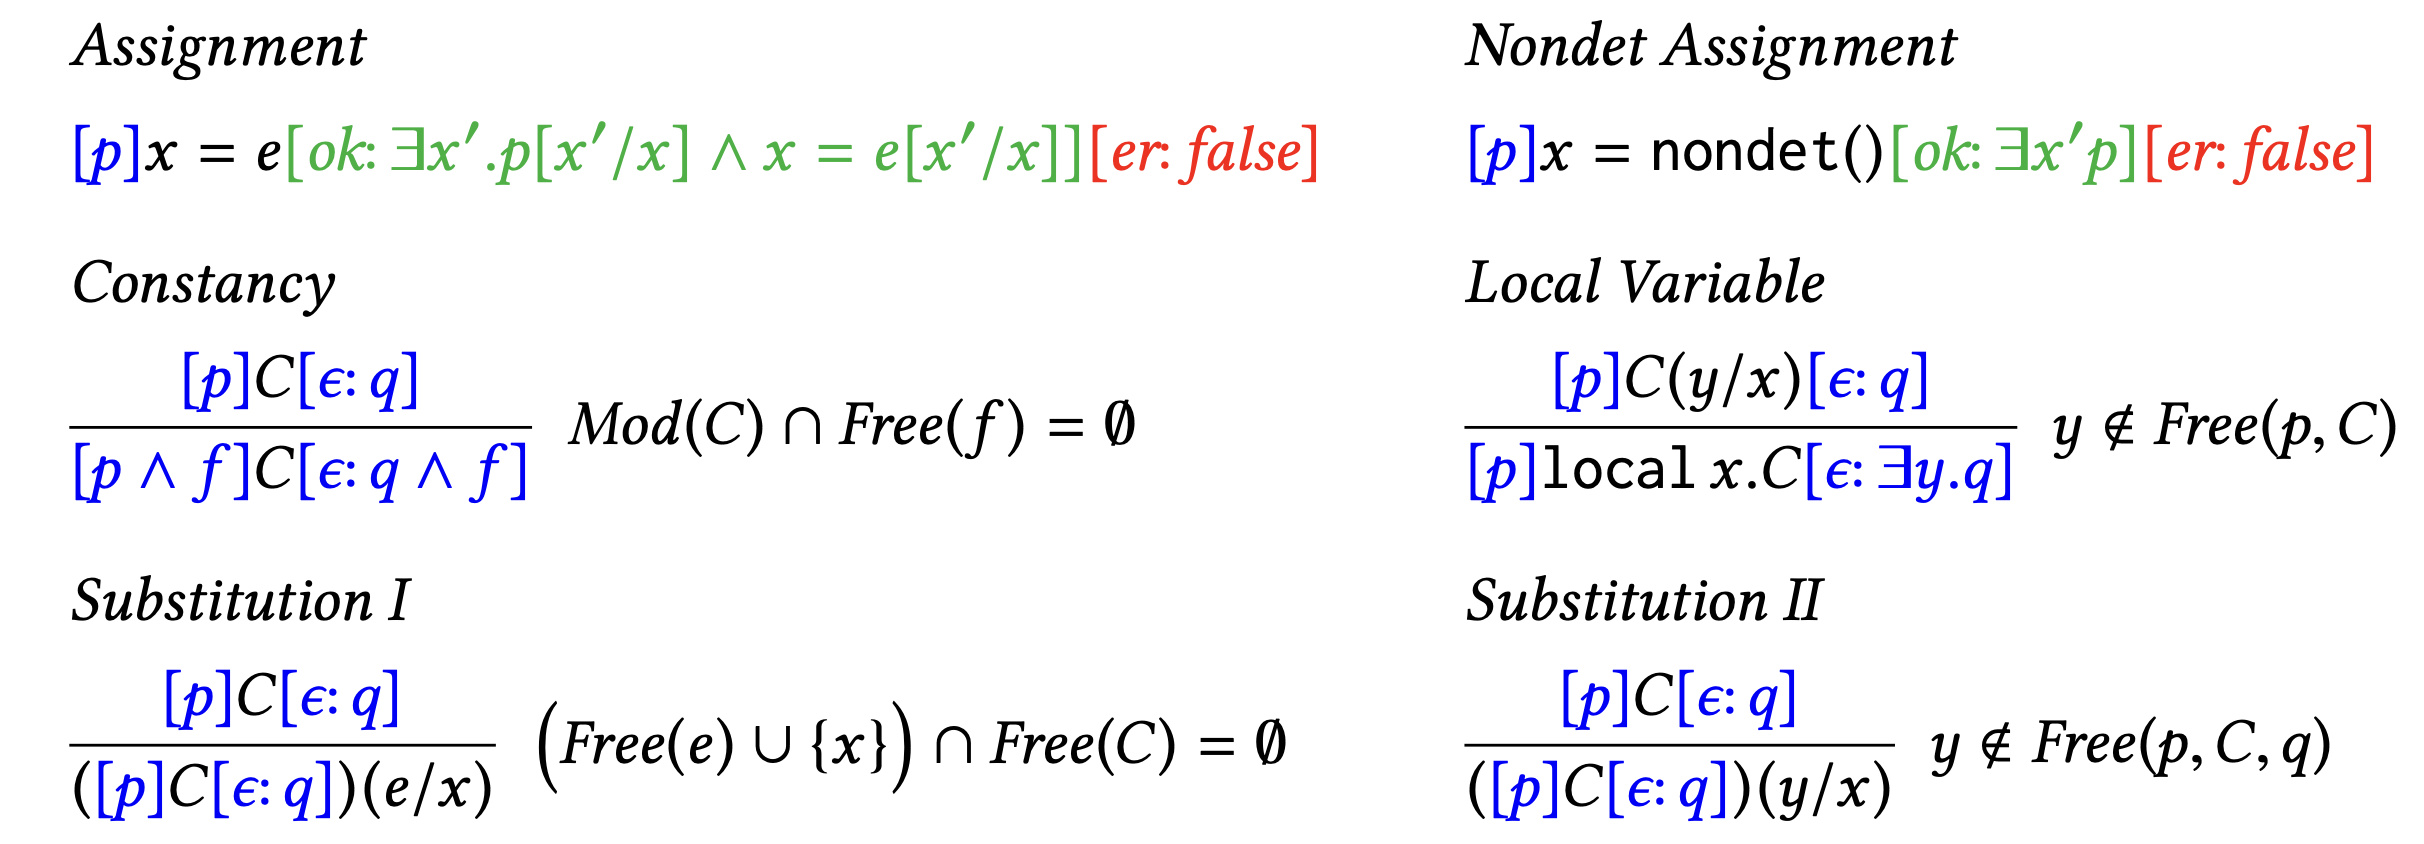
\includegraphics[width=\textwidth,height=0.3\textheight]{images/specific.png}
\caption{Rules for Variables and Mutation (Source:
\href{https://dl.acm.org/doi/10.1145/3371078}{Incorrectness Logic
Paper})}
\end{figure}

\begin{itemize}
\item
  Sound when states are functions of type \(\Vars \to \Vals\).
\item
  \emph{Mod}\((C)\) is the set of variables modified by assignment
  statements in \(C\), and \emph{Free}\((r)\) is the set of free
  variables in an assertion \(r\).
\item
  \texttt{e} and \texttt{nondet()} are syntactically distinct.

  \begin{itemize}
  \tightlist
  \item
    \texttt{e} is an expression built up from a first-order logic
    signature, can appear within assertions, and is side-effect free.
  \item
    \texttt{nondet()} does not appear in assertions.
    \red{[BUG] in \emph{Nondet Assignment} rule}
  \end{itemize}
\end{itemize}
\end{frame}

\begin{frame}[fragile]{Specific Proof Rules - Assignment}
\phantomsection\label{specific-proof-rules---assignment}
\begin{itemize}
\tightlist
\item
  Incorrectness logic uses Floyd's forward-running assignment axiom
  rather than Hoare's backwards-running one.
\end{itemize}

\[
\inference[Assignment]{}{
    \ruleboth{p}{x = e}{\exists x' \,.\, p[x' / x] \land x = e[x' / x]}{\false}
}
\]

\begin{itemize}
\tightlist
\item
  Would the below rule be correct?
\end{itemize}

\[
\inference[Assignment']{}{
    \ruleboth{p[e / x]}{x = e}{p}{\false}
}
\]

\pause

\begin{itemize}
\tightlist
\item
  No! For example, \(\ruleok{y == 42}{x = 42}{x == y}\) is not valid
  (take the post-state \texttt{{[}x\ :\ 3,\ y\ :\ 3{]}}).
\end{itemize}
\end{frame}

\begin{frame}{Specific Proof Rules - Substitution, Constancy, \& Local
Variable Rule}
\phantomsection\label{specific-proof-rules---substitution-constancy-local-variable-rule}
\begin{center}
\begin{tabular}{cc}
    \emph{Substitution I} & \emph{Constancy} \\
    $(\Free(e) \cup \{x\}) \cap \Free(C) = \emptyset$ &
    $\Mod(C) \cap \Free(f) = \emptyset$ \\ & \\
    \inference[]{ \ruleeps{p}{C}{q} }{ (\ruleeps{p}{C}{q})(e / x) } &
    \inference[]{ \ruleeps{p}{C}{q} }{ \ruleeps{p \land f}{C}{q \land f} } \\ & \\
    \emph{Substitution II} & \emph{Local Variable} \\
    $y \not\in \Free(p,C,q)$ & $y \not\in \Free(p,C)$ \\ & \\
    \inference[]{ \ruleeps{p}{C}{q} }{ (\ruleeps{p}{C}{q})(y / x) } &
    \inference[]{ \ruleeps{p}{C (y/x)}{q} }{ \ruleeps{p}{\local x \,.\, C}{\exists y \,.\, q} }
\end{tabular}
\end{center}

\begin{itemize}
\tightlist
\item
  The rules of \emph{Substitution}, \emph{Constancy} \&
  \emph{Consequence} are important for adapting specifications for use
  in different contexts.
\end{itemize}
\end{frame}

\begin{frame}[fragile]{Exercise: Derive rules for \texttt{assert}}
\phantomsection\label{exercise-derive-rules-for-assert}
\begin{itemize}
\tightlist
\item
  Recall \texttt{assert(B)\ =\ assume(B)\ +\ (assume(!B)\ ;\ error())}
\end{itemize}

\[
\ruleboth{p \land B}{\texttt{assert}(B)}{(p \land B)}{\false}
\]

\[
\ruleboth{p \land \neg B}{\texttt{assert}(B)}{\false}{(p \land \neg B)}
\]

\[
\ruleboth{p}{\texttt{assert}(B)}{(p \land B)}{(p \land \neg B)}
\]
\end{frame}

\section{Reasoning with the Logic}\label{reasoning-with-the-logic}

\begin{frame}[fragile]{Setup}
\phantomsection\label{setup-1}
\begin{itemize}
\item
  Examples motivated by existing tools, \emph{but} ``we are not claiming
  at this time that incorrectness logic leads to better practical
  results than these mature tools''
\item
  \emph{`A basic test of a potential foundational formalism is how it
  expresses a variety of patterns that have arisen naturally.'}
\item
  No formal treatment of procedures. Assume summary-like hypotheses for
  reasoning. \[
    \ruleboth{p}{\texttt{foo()}}{q}{r} \vdash \ruleboth{p'}{C}{q'}{r'}
    \]
\item
  \emph{Principle of reuse}: Reason about \texttt{foo()}'s body once,
  don't revisit at call sites (aka summary-based analysis -
  \href{iitd.github.io/col729}{COL729} throwback)
\end{itemize}
\end{frame}

\begin{frame}[fragile]{\texttt{loop0} - I}
\phantomsection\label{loop0---i}
\begin{Shaded}
\begin{Highlighting}[]
\DataTypeTok{void}\NormalTok{ loop0}\OperatorTok{()} \OperatorTok{\{}
    \CommentTok{/* (default presumes is "true" when not specified)}
\CommentTok{     * achieves: [ok: x\textgreater{}=0 ] */}
    \DataTypeTok{int}\NormalTok{ n }\OperatorTok{=}\NormalTok{ nondet}\OperatorTok{();}
\NormalTok{    x}\OperatorTok{=}\DecValTok{0}\OperatorTok{;}
    \ControlFlowTok{while} \OperatorTok{(}\NormalTok{n }\OperatorTok{\textgreater{}} \DecValTok{0}\OperatorTok{)} \OperatorTok{\{}
\NormalTok{        x }\OperatorTok{=}\NormalTok{ x }\OperatorTok{+}\NormalTok{ n}\OperatorTok{;}
\NormalTok{        n }\OperatorTok{=}\NormalTok{ nondet}\OperatorTok{();}
    \OperatorTok{\}\}}

\DataTypeTok{void}\NormalTok{ client0}\OperatorTok{()} \OperatorTok{\{} \CommentTok{/* achieves: [er: x==200000] */}
\NormalTok{    loop0}\OperatorTok{();}
    \ControlFlowTok{if} \OperatorTok{(}\NormalTok{x }\OperatorTok{==} \DecValTok{200000}\OperatorTok{)}\NormalTok{ error}\OperatorTok{();} \OperatorTok{\}}
\end{Highlighting}
\end{Shaded}

\begin{itemize}
\tightlist
\item
  Assuming \texttt{loop0} summary, can prove \texttt{client0} spec using
  below followed by sequencing rule. \[
    \inference[]{\ruleok{\true}{\texttt{loop0()}}{x \geq 0} \quad x \geq 0 \simpliedby x == 200000}{\ruleok{\true}{\texttt{loop0()}}{x == 200000}}
    \]
\end{itemize}
\end{frame}

\begin{frame}[fragile]{\texttt{loop0} - II}
\phantomsection\label{loop0---ii}
\begin{itemize}
\tightlist
\item
  How to prove \texttt{loop0()} spec?
\end{itemize}

\pause

\begin{itemize}
\tightlist
\item
  Just unroll once! Then apply \emph{Local Variable} rule +
  \emph{Unrolling} rule + \emph{Rule of Consequence}.
\end{itemize}

\begin{Shaded}
\begin{Highlighting}[]
\OperatorTok{[}\NormalTok{ x}\OperatorTok{==}\DecValTok{0} \OperatorTok{]}
    \ControlFlowTok{if} \OperatorTok{(}\NormalTok{n}\OperatorTok{\textgreater{}}\DecValTok{0}\OperatorTok{)} \OperatorTok{\{}
        \OperatorTok{[}\NormalTok{ x}\OperatorTok{==}\DecValTok{0} \OperatorTok{\&\&}\NormalTok{ n}\OperatorTok{\textgreater{}}\DecValTok{0} \OperatorTok{]}
\NormalTok{        x }\OperatorTok{=}\NormalTok{ x}\OperatorTok{+}\NormalTok{n}\OperatorTok{;}\NormalTok{ n }\OperatorTok{=}\NormalTok{ nondet}\OperatorTok{();} \OperatorTok{[}\NormalTok{ x}\OperatorTok{\textgreater{}}\DecValTok{0} \OperatorTok{]}
    \OperatorTok{\}} \ControlFlowTok{else}
    \OperatorTok{\{} \OperatorTok{[}\NormalTok{ x}\OperatorTok{==}\DecValTok{0} \OperatorTok{\&\&}\NormalTok{ n}\OperatorTok{\textless{}=}\DecValTok{0} \OperatorTok{]}\NormalTok{ skip}\OperatorTok{;}
    \OperatorTok{\}}
    \OperatorTok{[}\NormalTok{ x}\OperatorTok{\textgreater{}}\DecValTok{0} \OperatorTok{||} \OperatorTok{(}\NormalTok{x}\OperatorTok{==}\DecValTok{0} \OperatorTok{\&\&}\NormalTok{ n}\OperatorTok{\textless{}=}\DecValTok{0}\OperatorTok{)} \OperatorTok{]}
\NormalTok{        assume }\OperatorTok{(}\NormalTok{n}\OperatorTok{\textless{}=}\DecValTok{0}\OperatorTok{);}
    \OperatorTok{[} \OperatorTok{(}\NormalTok{x}\OperatorTok{\textgreater{}}\DecValTok{0} \OperatorTok{\&\&}\NormalTok{ n}\OperatorTok{\textless{}=}\DecValTok{0}\OperatorTok{)} \OperatorTok{||} \OperatorTok{(}\NormalTok{x}\OperatorTok{==}\DecValTok{0} \OperatorTok{\&\&}\NormalTok{ n}\OperatorTok{\textless{}=}\DecValTok{0}\OperatorTok{)} \OperatorTok{]}
\OperatorTok{[}\NormalTok{ ok}\OperatorTok{:}\NormalTok{ x}\OperatorTok{\textgreater{}=}\DecValTok{0} \OperatorTok{\&\&}\NormalTok{ n}\OperatorTok{\textless{}=}\DecValTok{0} \OperatorTok{]}
\end{Highlighting}
\end{Shaded}
\end{frame}

\begin{frame}[fragile]{\texttt{loop1} - I}
\phantomsection\label{loop1---i}
\begin{Shaded}
\begin{Highlighting}[]
\DataTypeTok{void}\NormalTok{ loop1}\OperatorTok{()}
\CommentTok{/*  achieves1: [ok: x==0 || x==1 || x==2]}
\CommentTok{    achieves2: [ok: x\textgreater{}=0] */}
\OperatorTok{\{}\NormalTok{   x }\OperatorTok{=} \DecValTok{0}\OperatorTok{;}
\NormalTok{    Kleene}\OperatorTok{{-}}\NormalTok{star }\OperatorTok{\{}
\NormalTok{        x }\OperatorTok{=}\NormalTok{ x }\OperatorTok{+} \DecValTok{1}\OperatorTok{;}
\OperatorTok{\}}   \OperatorTok{\}}

\DataTypeTok{void}\NormalTok{ client1}\OperatorTok{()}
\CommentTok{/* achieves: [er: x==200000] */}
\OperatorTok{\{}\NormalTok{   loop1}\OperatorTok{();}
    \ControlFlowTok{if} \OperatorTok{(}\NormalTok{ x}\OperatorTok{==}\DecValTok{200000} \OperatorTok{)}\NormalTok{ error}\OperatorTok{();}
\OperatorTok{\}}
\end{Highlighting}
\end{Shaded}
\end{frame}

\begin{frame}[fragile]{\texttt{loop1} - II}
\phantomsection\label{loop1---ii}
\begin{itemize}
\item
  Infinitely many paths through \texttt{loop1()}, and the loop is not
  guaranteed to terminate.
\item
  \emph{Unrolling} rule: post-conditions for any finite-depth unrollings
  of the loop. \texttt{achieves1}==2 unrollings.
\item
  Not enough to trigger the error in \texttt{client1()}. (Unroll 200000
  times?)
\item
  Need the backwards variant rule!
\end{itemize}

\[
\inference[$n$ fresh]{\ruleok{x==n \land \Nat(n)}{x = x+1}{ x == n+1 \land \Nat(n) }}{\ruleok{x==0}{(x = x+1)^{*}}{\exists n \,.\, x==n \land \Nat(n)}}
\]
\end{frame}

\begin{frame}[fragile]{\texttt{loop2} - I}
\phantomsection\label{loop2---i}
\begin{itemize}
\tightlist
\item
  Error inside iteration: This is why we need \(C^{*};C\), not
  \(C; C^{*}\)!
\end{itemize}

\begin{Shaded}
\begin{Highlighting}[]
\DataTypeTok{void}\NormalTok{ loop2}\OperatorTok{()}
\CommentTok{/* achieves: [er: x==200000] */}
\OperatorTok{\{}\NormalTok{   x }\OperatorTok{=} \DecValTok{0}\OperatorTok{;}
\NormalTok{    Kleene}\OperatorTok{{-}}\NormalTok{star}\OperatorTok{\{}
        \ControlFlowTok{if} \OperatorTok{(}\NormalTok{x}\OperatorTok{==}\DecValTok{200000}\OperatorTok{)}\NormalTok{ error}\OperatorTok{();}
\NormalTok{        x }\OperatorTok{=}\NormalTok{ x }\OperatorTok{+} \DecValTok{1}\OperatorTok{;}
\OperatorTok{\}}   \OperatorTok{\}}
\end{Highlighting}
\end{Shaded}

\begin{itemize}
\tightlist
\item
  How can we show this?
\end{itemize}
\end{frame}

\begin{frame}{\texttt{loop2} - II}
\phantomsection\label{loop2---ii}
\begin{itemize}
\tightlist
\item
  Use \emph{Backwards Variant} rule
  (\(p(n) = 0 \leq x \leq 200000 \land x==n\)). \[
    \ruleok{x==0}{(\Body)^{*}}{0 \leq x \leq 200000} 
    \] \[
    \ruleok{x==0}{(\Body)^{*}}{x == 200000}
    \]
\end{itemize}

\pause

\begin{itemize}
\tightlist
\item
  \emph{Assume} + \emph{Error} + \emph{Sequencing} +
  \emph{Short-Circuit} gives us \[
    \ruleer{x==200000}{\Body}{x==200000}
    \]
\end{itemize}

\pause

\begin{itemize}
\tightlist
\item
  \emph{Sequencing} \[
    \ruleer{x==0}{(\Body)^{*} ; \Body}{x==200000}
    \]
\end{itemize}

\pause

\begin{itemize}
\tightlist
\item
  \emph{Iterate non-zero} \[
    \ruleer{x==0}{(\Body)^{*}}{x==200000}
    \]
\end{itemize}
\end{frame}

\begin{frame}[fragile]{\texttt{loop3}}
\phantomsection\label{loop3}
\begin{itemize}
\tightlist
\item
  What if we used \(C ; C^{*}\)? The proof for \texttt{loop2()} spec
  would have 200000 applications of \emph{Sequencing}.
\end{itemize}

\begin{Shaded}
\begin{Highlighting}[]
\DataTypeTok{void}\NormalTok{ loop3}\OperatorTok{()}
\CommentTok{/* achieves: [er: \textbackslash{}exists n (x==n /\textbackslash{} n \textless{}= 200000)] */}
\OperatorTok{\{}\NormalTok{ y }\OperatorTok{=}\NormalTok{ nondet}\OperatorTok{();}
\NormalTok{  x }\OperatorTok{=} \DecValTok{0}\OperatorTok{;}
\NormalTok{  Kleene}\OperatorTok{{-}}\NormalTok{star }\OperatorTok{\{}
    \ControlFlowTok{if} \OperatorTok{(}\NormalTok{y }\OperatorTok{==} \DecValTok{200000}\OperatorTok{)}\NormalTok{ error}\OperatorTok{();} 
\NormalTok{    x }\OperatorTok{=}\NormalTok{ x }\OperatorTok{+} \DecValTok{1}\OperatorTok{;}
\NormalTok{    y }\OperatorTok{=}\NormalTok{ y }\OperatorTok{+} \DecValTok{1}\OperatorTok{;}
\OperatorTok{\}} \OperatorTok{\}}
\end{Highlighting}
\end{Shaded}

\pause

\begin{itemize}
\tightlist
\item
  We don't know the number of iterations it'll take to get an error, and
  cannot prove the \texttt{er} assertion with finitely many unrollings.
\end{itemize}

\pause

\begin{itemize}
\tightlist
\item
  But we can be \texttt{cool} and use \emph{Backwards Variant} to derive
  more general under-approximate assertions than unrolling, and use the
  original \emph{Iterate non-zero} to derive an error from the general
  assertion (with just one \(C\) statement).
\end{itemize}
\end{frame}

\begin{frame}{Conditionals}
\phantomsection\label{conditionals}
\begin{itemize}
\tightlist
\item
  Use of Boolean conditions that are difficult for current theorem
  provers to deal with causes expressiveness issues.

  \begin{itemize}
  \tightlist
  \item
    E.g. multiplication goes beyond the decidable subsets of arithmetic
    encoded in automatic theorem provers.
  \end{itemize}
\item
  How do tools deal with this? And how can Incorrectness Logic deal with
  this?
\end{itemize}
\end{frame}

\begin{frame}[fragile]{Conditionals - Approach I}
\phantomsection\label{conditionals---approach-i}
\begin{Shaded}
\begin{Highlighting}[]
\DataTypeTok{int}\NormalTok{ difficult}\OperatorTok{(}\DataTypeTok{int}\NormalTok{ y}\OperatorTok{)}
\OperatorTok{\{}   \ControlFlowTok{return} \OperatorTok{(}\NormalTok{y}\OperatorTok{*}\NormalTok{y}\OperatorTok{);} \CommentTok{/* or hash(y) or obfuscated code */}
\OperatorTok{\}}

\DataTypeTok{void}\NormalTok{ client}\OperatorTok{()}
\CommentTok{/* achieves1 : [ok: y==49 \&\& x==1] */}
\OperatorTok{\{}   \DataTypeTok{int}\NormalTok{ z }\OperatorTok{=}\NormalTok{ nondet}\OperatorTok{();}
    \ControlFlowTok{if} \OperatorTok{(}\NormalTok{y }\OperatorTok{==}\NormalTok{ difficult}\OperatorTok{(}\NormalTok{z}\OperatorTok{))}
\NormalTok{        x}\OperatorTok{=}\DecValTok{1}\OperatorTok{;}
    \ControlFlowTok{else}
\NormalTok{        x}\OperatorTok{=}\DecValTok{2}\OperatorTok{;}
\OperatorTok{\}}
\end{Highlighting}
\end{Shaded}

\begin{itemize}
\item
  Pragmatic Approach from Dynamic Symbolic Execution: \emph{Concretize
  symbolic variables}. (replace \(z\) with \(7\)).
\item
  Do this in incorrectness logic by \emph{shrinking the post}. Have
  \texttt{{[}y==z*z{]}\ assume(y==difficult(z))\ {[}ok:\ y==z*z{]}} and
  \(y == z*z \simpliedby y==z*z \land z==7\).
\end{itemize}
\end{frame}

\begin{frame}[fragile]{Conditionals - Approach II}
\phantomsection\label{conditionals---approach-ii}
\begin{Shaded}
\begin{Highlighting}[]
\DataTypeTok{void}\NormalTok{ client}\OperatorTok{()}
\CommentTok{/* achieves2 : [ok: exists z . (y==difficult(z) \&\& x==1)}
\CommentTok{    || (y!=difficult(z) \&\& x==2)] */}
\OperatorTok{\{}   \DataTypeTok{int}\NormalTok{ z }\OperatorTok{=}\NormalTok{ nondet}\OperatorTok{();}
    \ControlFlowTok{if} \OperatorTok{(}\NormalTok{y }\OperatorTok{==}\NormalTok{ difficult}\OperatorTok{(}\NormalTok{z}\OperatorTok{))}
\NormalTok{        x}\OperatorTok{=}\DecValTok{1}\OperatorTok{;}
    \ControlFlowTok{else}
\NormalTok{        x}\OperatorTok{=}\DecValTok{2}\OperatorTok{;}
\OperatorTok{\}}

\DataTypeTok{void}\NormalTok{ test1}\OperatorTok{()}
\CommentTok{/* achieves: [er: exists z .}
\CommentTok{    (y==difficult(z) \&\& x==1)}
\CommentTok{    || (y != difficult(z) \&\& x==2)] */}
\OperatorTok{\{}\NormalTok{   client}\OperatorTok{();} \ControlFlowTok{if} \OperatorTok{(}\NormalTok{x}\OperatorTok{==}\DecValTok{1} \OperatorTok{||}\NormalTok{ x}\OperatorTok{==}\DecValTok{2}\OperatorTok{)}\NormalTok{ error}\OperatorTok{();}
\OperatorTok{\}}
\end{Highlighting}
\end{Shaded}

\begin{itemize}
\tightlist
\item
  Record information lazily (hoping difficulty won't matter, like in
  \texttt{test1()}).
\end{itemize}
\end{frame}

\begin{frame}[fragile]{Conditionals - Approach III}
\phantomsection\label{conditionals---approach-iii}
\begin{Shaded}
\begin{Highlighting}[]
\DataTypeTok{void}\NormalTok{ client}\OperatorTok{()}
\CommentTok{/* achieves3 : [ok: x==1 || x==2] */}
\OperatorTok{\{}   \DataTypeTok{int}\NormalTok{ z }\OperatorTok{=}\NormalTok{ nondet}\OperatorTok{();}
    \ControlFlowTok{if} \OperatorTok{(}\NormalTok{y }\OperatorTok{==}\NormalTok{ difficult}\OperatorTok{(}\NormalTok{z}\OperatorTok{))}
\NormalTok{        x}\OperatorTok{=}\DecValTok{1}\OperatorTok{;}
    \ControlFlowTok{else}
\NormalTok{        x}\OperatorTok{=}\DecValTok{2}\OperatorTok{;}
\OperatorTok{\}}

\DataTypeTok{void}\NormalTok{ test2}\OperatorTok{()}
\OperatorTok{\{}\NormalTok{   client}\OperatorTok{();} \ControlFlowTok{if} \OperatorTok{(}\NormalTok{x}\OperatorTok{==}\DecValTok{2}\OperatorTok{)}\NormalTok{ error}\OperatorTok{();} \OperatorTok{\}}
\end{Highlighting}
\end{Shaded}

\begin{itemize}
\item
  Record disjuncts for both branches, but discard the difficult bits.
  \red{Unsound!} (e.g.~\texttt{{[}x:1,\ y:3{]}} not reachable).
\item
  Used for pragmatic reasons in tools like SMART, Infer.RacerD.
\item
  RacerD: it is \emph{an under-approximation of an over-approximation},
  where the over-approximation arises by replacing Booleans it doesn't
  understand with nondeterministic choice.
\end{itemize}
\end{frame}

\begin{frame}[fragile]{Tool Design Insights}
\phantomsection\label{tool-design-insights}
\begin{itemize}
\item
  \texttt{Infer.RacerD}: Tools can make localised unsound decisions,
  which act as assumptions for further sound steps.
\item
  \emph{`From this perspective, the role of logic is not to produce
  iron-clad unconditional guarantees, but is to clarify assumptions and
  their role when making sound inferences.'}
\item
  \texttt{Infer.Pulse}: 20 disjuncts case was \textasciitilde2.75x wall
  clock time faster, \textasciitilde3.1x user time faster, and found
  97\% of the issues that the 50 disjuncts case found.

  \begin{itemize}
  \tightlist
  \item
    Choice is not binary! E.g., deploy fast one at code review time,
    slow one later in the process.
  \end{itemize}
\end{itemize}
\end{frame}

\begin{frame}{Flaky Tests - I}
\phantomsection\label{flaky-tests---i}
\begin{itemize}
\item
  ``flaky test'' : due to nondeterminism, can give different answers on
  different runs.
\item
  If \(\pi\) is a program path, then

  \begin{itemize}
  \tightlist
  \item
    \(\Wp(\pi)q\): States for which execution of \(\pi\) is guaranteed
    to terminate and satisfy \(q\).
  \item
    \(\Wpp(\pi)q\): States for which execution of \(\pi\) is possible to
    terminate and satisfy \(q\).
  \end{itemize}
\item
  We will use these to obtain pre-assertions, then use forward reasoning
  to obtain under-approximate post-assertions.
\item
  Why do we need these?

  \begin{itemize}
  \tightlist
  \item
    Because strongest under-approximate presumptions do not exist in
    general (see 5.2 in paper).
  \end{itemize}
\end{itemize}
\end{frame}

\begin{frame}[fragile]{Flaky Tests - II}
\phantomsection\label{flaky-tests---ii}
\begin{Shaded}
\begin{Highlighting}[]
\DataTypeTok{void}\NormalTok{ foo}\OperatorTok{()}
\CommentTok{/* sturdy pre [x is even], ach [er: x is even][ok: false]}
\CommentTok{    flaky pre [x is odd], ach [er: x is odd][ok: x is odd] */}
\OperatorTok{\{}
    \ControlFlowTok{if} \OperatorTok{(}\NormalTok{x is even}\OperatorTok{)}\NormalTok{ error}\OperatorTok{();}
    \ControlFlowTok{else} \OperatorTok{\{} \ControlFlowTok{if} \OperatorTok{(}\NormalTok{nondet}\OperatorTok{())}\NormalTok{ skip}\OperatorTok{;} \ControlFlowTok{else}\NormalTok{ error}\OperatorTok{();} \OperatorTok{\}}
\OperatorTok{\}}

\DataTypeTok{void}\NormalTok{ flakey\_client}\OperatorTok{()}
\CommentTok{/* flaky achieves: [er: x==3 || x==5] */}
\OperatorTok{\{}\NormalTok{   x }\OperatorTok{=} \DecValTok{3}\OperatorTok{;}
\NormalTok{    foo}\OperatorTok{();}
\NormalTok{    x }\OperatorTok{=}\NormalTok{ x}\OperatorTok{+}\DecValTok{2}\OperatorTok{;}
\NormalTok{    assert}\OperatorTok{(}\NormalTok{x}\OperatorTok{==}\DecValTok{4}\OperatorTok{);}
\OperatorTok{\}}
\end{Highlighting}
\end{Shaded}

\begin{itemize}
\item
  Use \(\Wp(\Assume (x \texttt{ is even})) \; \true\) for sturdy
  presumes,
  \(\Wpp(\Assume(x \texttt{ is odd}); b=\texttt{nondet}(); \Assume ( b )) \; \true\)
  (where \(b\) is local) for flaky presumes.
\item
  A proof of incorrectness can be checked repeatedly in a deterministic
  fashion. (unclear if this helps)
\end{itemize}
\end{frame}

\begin{frame}{Reasoning about Procedures - I}
\phantomsection\label{reasoning-about-procedures---i}
\begin{itemize}
\item
  For a path without procedure calls - say a sequential composition of
  assignment, assume and assert statements

  \begin{itemize}
  \tightlist
  \item
    Can perform strongest post-condition reasoning, which is also
    under-approximate.
  \end{itemize}
\item
  Can combine together pre/post pairs for a number of paths to get an
  under-approximate summary for a procedure.
\item
  But then using that summary to reason (\emph{soundly}) about a path
  containing a procedure call is subtle.
\item
  Even in straight-line code, it is \emph{easy} to get a false positive
  using strongest post-condition reasoning with Hoare logic.
\end{itemize}
\end{frame}

\begin{frame}[fragile]{Reasoning about Procedures - II}
\phantomsection\label{reasoning-about-procedures---ii}
\begin{Shaded}
\begin{Highlighting}[]
\DataTypeTok{void}\NormalTok{ inc}\OperatorTok{()}
\CommentTok{/* presumes1: [x\textgreater{}=0], achieves1: [ok: x\textgreater{}0]}
\CommentTok{   presumes2: [x==m \&\& m\textgreater{}=0], achieves2: [ok: x==m+1 \&\& m\textgreater{}=0] */}
\OperatorTok{\{}\NormalTok{   assert}\OperatorTok{(}\NormalTok{x}\OperatorTok{\textgreater{}=}\DecValTok{0}\OperatorTok{);}
\NormalTok{    x}\OperatorTok{=}\NormalTok{x}\OperatorTok{+}\DecValTok{1}\OperatorTok{;}
\OperatorTok{\}}

\DataTypeTok{void}\NormalTok{ client}\OperatorTok{()}
\CommentTok{/* presumes1: [x\textgreater{}=0], wrong achieves1: [ok: x\textgreater{}0]}
\CommentTok{   presumes2: [x==m \&\& m\textgreater{}=0], achieves2: [ok: x==m+2 \&\& m\textgreater{}=0] */}
\OperatorTok{\{}\NormalTok{   inc}\OperatorTok{();}\NormalTok{ inc}\OperatorTok{();} \OperatorTok{\}}

\DataTypeTok{void}\NormalTok{ test}\OperatorTok{()}
\CommentTok{/* wrong achieves1: [er: x==1]}
\CommentTok{   achieves2: [er: false] */}
\OperatorTok{\{}\NormalTok{   x }\OperatorTok{=} \DecValTok{0}\OperatorTok{;}
\NormalTok{    client}\OperatorTok{();}
\NormalTok{    assert}\OperatorTok{(}\NormalTok{x}\OperatorTok{\textgreater{}=}\DecValTok{2}\OperatorTok{);}
\OperatorTok{\}}
\end{Highlighting}
\end{Shaded}
\end{frame}

\begin{frame}[fragile]{Reasoning about Procedures - III}
\phantomsection\label{reasoning-about-procedures---iii}
\begin{itemize}
\item
  Incorrectness logic prevents the unsound (for bug catching) inference
  \texttt{presumes1/achieves1} for \texttt{client()} and thus
  \texttt{test()}.
\item
  A different spec of \texttt{inc()}, given by
  \texttt{presumes2/achieves2}, lets us reason about the composition
  \texttt{inc();inc()} in \texttt{client()} more positively, to obtain
  \texttt{presumes2/achieves2} as stated for \texttt{client()}.
\item
  Note: A procedure spec or summary should carry information about free
  variables and modified - for \texttt{inc()}, \(x\) is free and
  modified, \(m\) is not free in the procedure body.
\item
  This allows us to apply rules of \emph{Substitution} and
  \emph{Constancy} to get \texttt{client()} spec from \texttt{inc()}
  spec.
\end{itemize}
\end{frame}

\begin{frame}[fragile]{Context and Conclusions}
\phantomsection\label{context-and-conclusions}
\begin{itemize}
\item
  \emph{`The theory Infer was based on originally \ldots{} does not
  match its use to find bugs rather than to prove their absence.'}
\item
  Led to \texttt{RacerD}, \texttt{Pulse} program analysers.
\item
  A more general theory of ``incorrectness'' logic (starting from
  reverse Hoare logic by de Vries and Koutavas in 2011).
\item
  Related theoretical notions: \texttt{wlp} (weakest liberal
  precondition), \texttt{wpp} (weakest possible precondition), dynamic
  logic.
\item
  Each form of reasoning is as fundamental as the other, they just have
  different principles. Recall:
\end{itemize}

\begin{quote}
For correctness reasoning, you \textbf{get to forget information} as you
go along a path, but you \textbf{must remember} all the paths. For
incorrectness reasoning, you \textbf{must remember} information as you
go along a path, but you \textbf{get to forget} some of the paths.
\end{quote}

\begin{itemize}
\tightlist
\item
  Possible extensions to other models, concurrency. Possible reuse of
  work from termination proving.
\end{itemize}

\begin{center}
    Thank You!
\end{center}
\end{frame}

\section{Appendix}\label{appendix}

\begin{frame}[fragile]{Backwards Variant - Example I}
\phantomsection\label{backwards-variant---example-i}
\begin{itemize}
\tightlist
\item
  For any fixed number of iterations, we can just unfold the
  \emph{Iterate non-zero} rule and use \emph{Iterate zero}. But no. of
  iterations may be unknown!
\end{itemize}

\begin{Shaded}
\begin{Highlighting}[]
\NormalTok{x }\OperatorTok{=} \DecValTok{0}\OperatorTok{;}
\NormalTok{y }\OperatorTok{=}\NormalTok{ nondet}\OperatorTok{();}
\ControlFlowTok{while} \OperatorTok{(}\NormalTok{y }\OperatorTok{!=}\NormalTok{ N}\OperatorTok{)} \ControlFlowTok{do} \OperatorTok{\{}
\NormalTok{    y }\OperatorTok{=}\NormalTok{ y }\OperatorTok{+} \DecValTok{1}\OperatorTok{;}
\NormalTok{    x }\OperatorTok{=}\NormalTok{ x }\OperatorTok{+} \DecValTok{1}\OperatorTok{;}
\OperatorTok{\}}
\end{Highlighting}
\end{Shaded}

\[
\ruleok{x = 0}{\texttt{while (y != N) do { y = y + 1; x = x + 1 }}}{\exists n \,.\, x == n \land \Nat(n)}
\]
\end{frame}

\begin{frame}[fragile]{Backwards Variant - Example II}
\phantomsection\label{backwards-variant---example-ii}
\begin{Shaded}
\begin{Highlighting}[]
\DataTypeTok{void}\NormalTok{ loop3}\OperatorTok{()}
\CommentTok{/* achieves: [er: x == 200000] */}
\OperatorTok{\{}\NormalTok{ x }\OperatorTok{=}\NormalTok{ nondet}\OperatorTok{();}
\NormalTok{  Kleene}\OperatorTok{{-}}\NormalTok{star }\OperatorTok{\{}
    \ControlFlowTok{if} \OperatorTok{(}\NormalTok{x }\OperatorTok{==} \DecValTok{200000}\OperatorTok{)}\NormalTok{ error}\OperatorTok{();} 
\NormalTok{    x }\OperatorTok{=}\NormalTok{ x }\OperatorTok{+} \DecValTok{1}\OperatorTok{;}
\OperatorTok{\}} \OperatorTok{\}}
\end{Highlighting}
\end{Shaded}

\pause

\begin{itemize}
\tightlist
\item
  Can guess a value \(k\) returned by \texttt{nondet()} and apply
  \emph{Sequencing} \(200000-k\) times. Or
\end{itemize}

\pause

\begin{itemize}
\tightlist
\item
  Can be \texttt{cool} and use \emph{Backwards Variant} to derive more
  general under-approximate assertions than unrolling, and use the
  original \emph{Iterate non-zero} to derive an error from the general
  assertion (with just one \(C\) statement).
\end{itemize}
\end{frame}

\end{document}
